% !TXS template
\documentclass[italian]{article}
\usepackage[T1]{fontenc}
\usepackage[utf8]{inputenc}
\usepackage{lmodern}
\usepackage[a4paper,top=2cm,bottom=2cm,left=1cm,right=1cm]{geometry}
\usepackage[italian]{babel}
\usepackage{enumitem}
\usepackage[fleqn]{amsmath}
\usepackage{amssymb}
\usepackage{mathtools}% http://ctan.org/pkg/mathtools
\usepackage{cancel}
\usepackage{color}
\usepackage[usenames,dvipsnames]{xcolor}
\usepackage{units}
\usepackage{hyperref}
\usepackage{textcomp}
\usepackage{soul}
\usepackage{tikz}
\usetikzlibrary{matrix,decorations.pathreplacing}
\usetikzlibrary{calc}
\usepackage{pifont} %https://www.rpi.edu/dept/arc/training/latex/LaTeX_symbols.pdf
\usepackage[customcolors]{hf-tikz} % http://tex.stackexchange.com/questions/69713/matrix-change-row-or-column-background

\hypersetup{
	colorlinks,
	citecolor=black,
	filecolor=black,
	linkcolor=black,
	urlcolor=black
}


\tikzset{style green/.style={
		set fill color=green!50!lime!60,
		set border color=white,
	},
	style cyan/.style={
		set fill color=cyan!90!blue!60,
		set border color=white,
	},
	style orange/.style={
		set fill color=orange!80!red!60,
		set border color=white,
	},
	hor/.style={
		above left offset={-0.15,0.31},
		below right offset={0.15,-0.125},
		#1
	},
	ver/.style={
		above left offset={-0.1,0.3},
		below right offset={0.15,-0.15},
		#1
	}
}

\newcommand{\tikzmark}[1]{\tikz[overlay,remember picture] \node (#1) {};}
\newcommand{\DrawLine}[3][]{%
	\begin{tikzpicture}[overlay,remember picture]
	\draw [#1] ($(#2)+(0,0.6ex)$) -- ($(#3)+(0,0.6ex)$);
	\end{tikzpicture}%
}%
\renewcommand{\labelitemii}{$\circ$}
\newcommand{\parallele}{\mathbin{\!/\mkern-5mu/\!}}

\newcommand\x{\times}
\newcommand{\linea}{\begin{center}\rule{5cm}{1pt}\end{center}}
\newcommand{\crossmark}{\textcolor{red}{\text{$\qquad$\ding{56}}}}
\renewcommand{\checkmark}{\textcolor{ForestGreen}{\text{$\qquad$\ding{52}}}}
\newcommand{\ins}[1]{\text{$\mathbb{#1}$}}
\newcommand{\tright}[1]{\hfill #1 \\}
\renewcommand{\dim}[1]{\text{dim$\left(#1\right)$}}
\renewcommand{\ker}[1]{\text{ker$\left(#1\right)$}}
\newcommand{\imm}[1]{\text{Imm$\left(#1\right)$}}
\renewcommand{\det}[1]{\text{det$\left(#1\right)$}}
\newcommand{\cof}[2]{\text{cof$_{#1}\left(#2\right)$}}
\newcommand{\rk}[1]{\text{rk$\left(#1\right)$}}

\newcommand\encircle[1]{%
	\tikz[baseline=(X.base)] 
	\node (X) [draw, shape=circle, inner sep=0] {\strut #1};}

\author{Giacomo De Liberali}





\begin{document}
	
\title{Alebra lineare}
\maketitle

\tableofcontents
\pagebreak

\section{Numeri complessi}
Un numero complesso è definito come: $z=a+bi$\\
La parte reale di $z$ è definita come: $Re(z)=a$\\
La parte immaginaria di $z$ è definita come: $Im(z)=b$ \\
Il modulo (o lunghezza) è definito come: $|z| = \sqrt{a^2+b^2}$\\\\
\textbf{Proprietà}\\
\begin{itemize}
	\item coniugato $\to \overline{z} = a - bi$	
	\item $\overline{z} \cdot \overline{z} = a^2+b^2$
	\item $z + \overline{z} = 2a = 2\cdot Re(z)$
	\item $z-\overline{z}=(a+bi)-(a-bi)=2bi = 2\cdot Im(z)$
	\item $|z|=|\overline{z}|$ \qquad \emph{[il modulo di un numero complesso è 0 solo quando anche z è 0]}
	\item $\overline{z1+z2}=\overline{z1}+\overline{z2}$
	\item $\overline{z1\cdot z2}=\overline{z1}\cdot \overline{z2}$
	\item $|z1+z2|\leq |z1|+|z2|$
\end{itemize}
\textbf{Argand - Gauss}\\
Su un piano ogni punto può essere rappresentato da una coppia di coordinate.\\
\begin{center}
	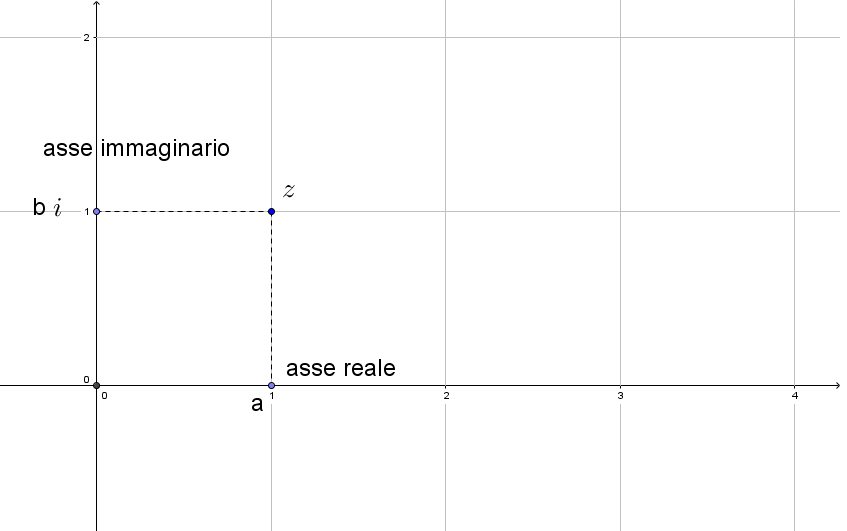
\includegraphics[width=0.5\linewidth]{img/argan_gauss}	
\end{center}
\pagebreak
\subsection{Applicazione numeri complessi}
\begin{center}
	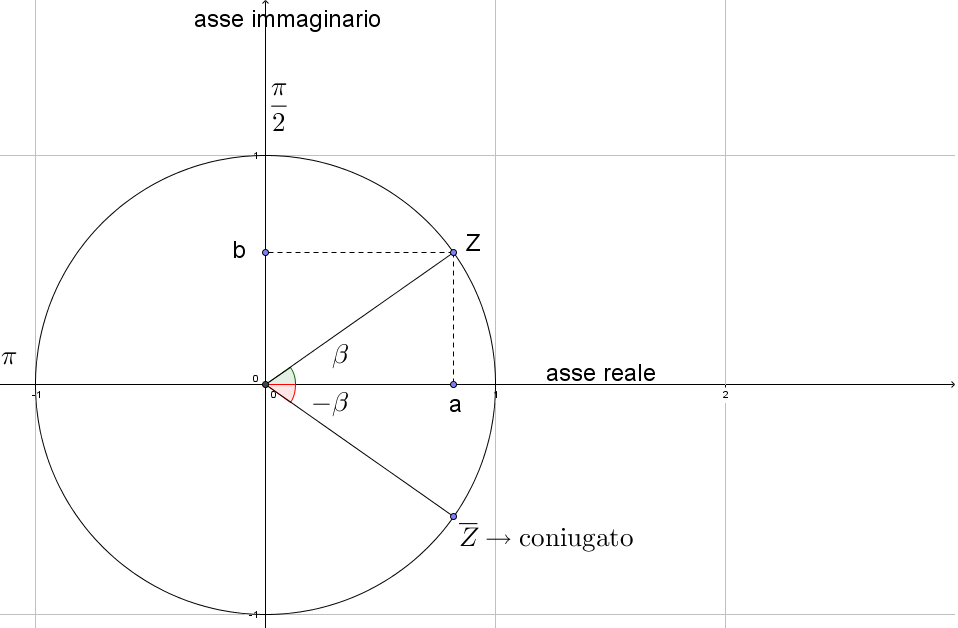
\includegraphics[width=0.5\linewidth]{img/numeri_compessi}	
\end{center}
Se $z$ si trova sulla circonferenza di raggio unitario e centro $(0,0)$ allora $z$ è definito come $z=\cos (\beta)+i\cdot \sin (\beta)$ dove $\beta$ è l'angolo formato dal raggio unitario (che parte da $(0,0)$ fino a $z$) e la sua proiezione sull'asse positivo reale. \\\\
Il modulo di un numero complesso è definito come la lunghezza del segmento di origine $(0,0)$ e termine $z$. Si calcola come segue:
\[
	|z|=\sqrt{\cos (\beta)^2 + \sin (\beta)^2} = 1
\]
Segue che $\cos ^2 \beta + \sin ^2 \beta = 1$. \\
Se la circonferenza fosse stata di raggio r=2, anche il modulo del numero complesso sarebbe stato 2. $\to u=2\cos \beta + 2i \cdot \sin \alpha$\\\\
\subsection{Moltiplicazioni tra numeri complessi}
Moltiplicare due numeri complessi tra loro significa sommare gli angoli.
\begin{center}
	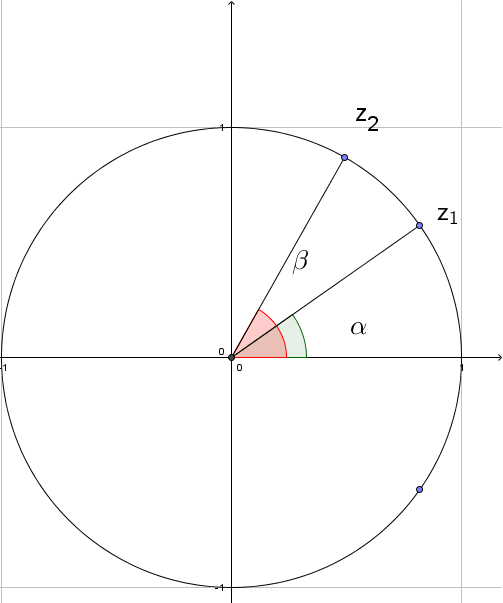
\includegraphics[width=0.3\linewidth]{img/numeri_compessi_1.png}	
\end{center}
$z_1 \cdot z_2 = \cos (\alpha + \beta) + \sin (\alpha + \beta)$\\\\
\pagebreak
\subsubsection{Rappresentazioni alternative}
$z_1$ può essere definito come: $|z_1|(\cos \alpha + i\sin \alpha)$, 
mentre $z_2$ può essere definito come: $|z_2|(\cos \beta + i\sin \beta)$.\\
Un numero complesso moltiplicato per il suo coniugato è uguale al quadrato del modulo:
\[
	z\cdot \overline{z} = |z|^2 = a^2 + b^2
\]
Il prodotto di due numeri complessi $z_1$ e $z_2$ è definito come segue:
\[
	z_1 \cdot z_2 = |z_1|\cdot |z_2|\cdot (\cos (\alpha + \beta) + i\cdot \sin (\alpha + \beta))
\]
L'inverso di un numero complesso $z$ è definito come:
\[
	z_1 = \rho \cdot (\cos \alpha + i\cdot \sin \beta) \qquad \text{dove $\rho$ è un numero reale qualsiasi}
\]
E si calcola come:
\begin{gather*}
	z\cdot \overline{z} = \rho ^2 \cdot 1 \\
	z^{-1} = \frac{\overline{z}}{\rho ^2}=\frac{\cos \alpha - i\cdot \sin \alpha}{\rho}
\end{gather*}

\subsubsection{Formula di Eulero}
\begin{gather*}
	e^{e\cdot t} \qquad \qquad \text{dove $t$ è un numero reale} \\
	e^{e\cdot t} = \cos (t) + i\cdot \sin (t) \\
	z=\rho \cdot e^{i\cdot t} \\
	e^z = e^{a+i\cdot b}=e^a\cdot e^{i\cdot b} = e^a\cdot (\cos b + i\cdot \sin b) \\
	e^{z+2k\pi \cdot i}=e^z\cdot \underbrace{e^{2k\pi \cdot i}}_{2k\pi \to angolo = 0} = e^z
\end{gather*}
\subsubsection{Esercizio}
\begin{gather*}
	z=i \to |i| = \sqrt{0^2 + 1^2} = 1\\\\ 
	i= \underbrace{\cos \beta}_{\frac{\pi}{2} \to 0} + i\cdot  \underbrace{\sin \beta}_{\frac{\pi}{2} \to 1} = i \\\\
	z=1+\textcolor{cyan}{1}\cdot i\\
	|z| = \sqrt{1^2+1^2}=\textcolor{red}{\sqrt{2}}\\
	z=\textcolor{red}{\sqrt{2}} \left( \frac{\textcolor{cyan}{1}}{\textcolor{red}{\sqrt{2}}}+\frac{\textcolor{cyan}{1}}{\textcolor{red}{\sqrt{2}}}\cdot i \right) 
\end{gather*}

\pagebreak
\section{Aritmetica modulare}
Nell'aritmetica modulare valgono le seguenti proprietà:
\begin{itemize}
	\item commutativa
	\item elemento neutro
	\item distribuiva del prodotto
	\item dell'opposto
	\item dell'inverso
\end{itemize}
\begin{align*}
	\text{SOMMA} && \text{PRODOTTO}\\
	0+0=0 && 0\cdot 0=0\\
	0+1=1 && 0\cdot 1=0\\
	1+0=1 && 1\cdot 0 = 0\\
	1+1=0 && 1\cdot 1=0
\end{align*}
\noindent\rule{8cm}{0.4pt} \\
$z = a + b\cdot i = |z|\cdot(\cos \alpha + i\cdot \sin \alpha)$
\begin{center}
	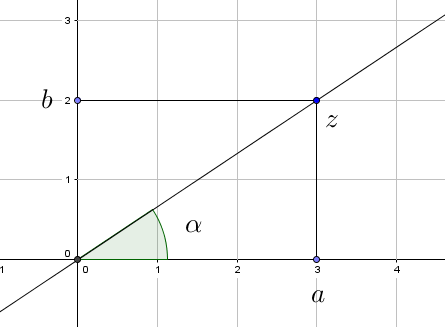
\includegraphics[width=0.3\linewidth]{img/vettori_0.png}	
\end{center}
Appena fisso un punto nel piano ottengo un segmento orientato che parte dell'origine e raggiunge il punto (in questo caso il punto P). Questo segmento prende il nome di \textbf{vettore}.\\
$z = (3,3) \to -1\cdot z = (-1\cdot 3, -1\cdot 3) = (-3,-3)$
\begin{center}
	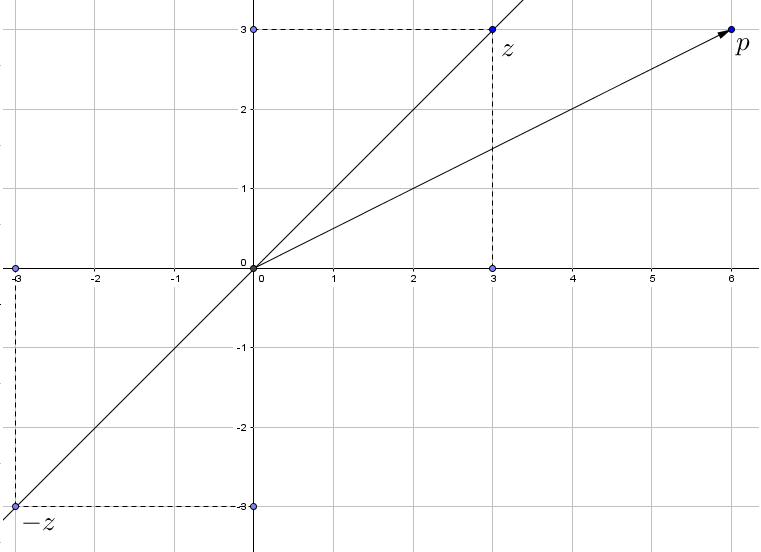
\includegraphics[width=0.4\linewidth]{img/vettori_-1.png}	
\end{center}
Moltiplicando un vettore per un numero reale $k$ cambio la lunghezza del vettore, ovvero la sua intensità. Nel caso in cui $k$ sia negativo, ottengo anche un cambiamento nella direzione del vettore. Il numero reale $k$ prende il nome di \textbf{scalare}.

\pagebreak
\section{Vettori}
I vettori sono una rappresentazione astratta delle grandezze che hanno una
direzione (e talvolta un verso).

\subsection{Somma vettoriale}
Nella somma fra vettori valgono le seguenti proprietà:
\begin{itemize}
	\item associativa
	\item commutativa
	\item elemento neutro
	\item opposto
\end{itemize}
Le somme di vettori costituiscono un \textbf{gruppo additivo} che è \textbf{commutativo}.\\
I vettori sono rappresentati per convenzione con lettere maiuscole, a differenza degli scalari che vengono rappresentati con le lettere minuscole.\\\\
\textbf{Esempi di proprietà}
\begin{gather*}
	(c+d)A = cA + dA\\
	(c\cdot d)A = (dA)\cdot c \\
	c\cdot (A+B)=cA + cB\\
	1 \cdot A = A \\
	0\cdot A = \underline{0} \to \text{sottolineo la scalare 0, \underline{non è un vettore}. Il vettore zero in un piano è definito come } A(0,0).
\end{gather*}
Lo spazio vettoriale su un campo numerico dipende da quale campo numerico sto utilizzando: se sto lavorando con i numeri complessi, lo spazio vettoriale sarà $\mathbb{C}$, oppure se sto lavorando con i numeri reali sarà $\mathbb{R}$ \dots\\\\
Rappresentazione grafica della somma vettoriale:
\begin{center}
	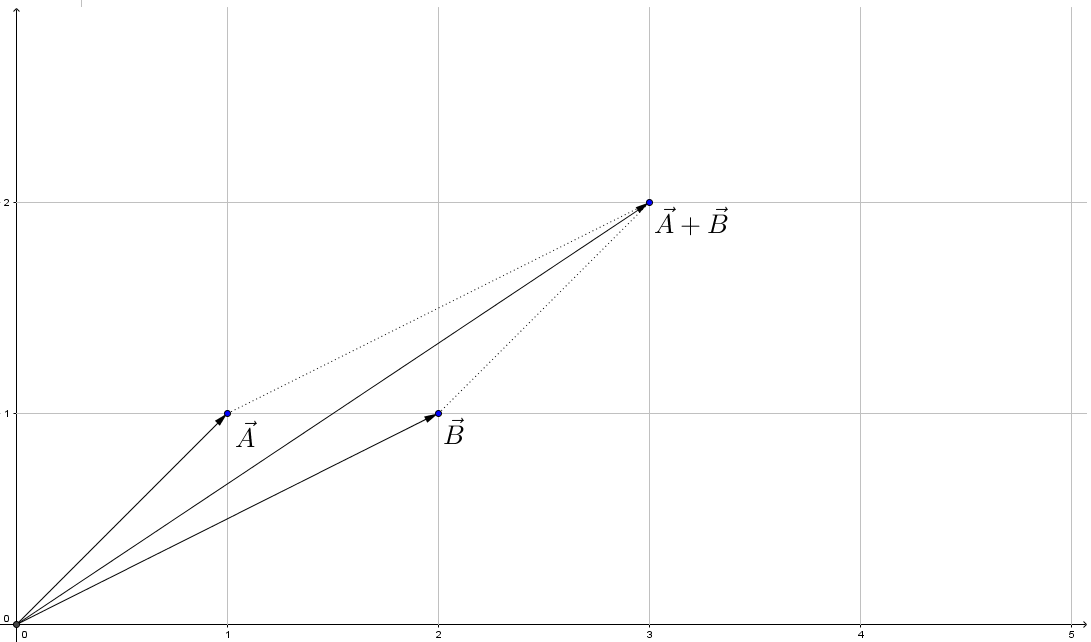
\includegraphics[width=0.6\linewidth]{img/vettori.png}	
\end{center}
\pagebreak
\subsection{Translazioni vettoriali}
Per traslazione di un vettore si intende il suo spostamento nel piano mantenendo inalterate direzione e intensità.\\
\begin{center}
	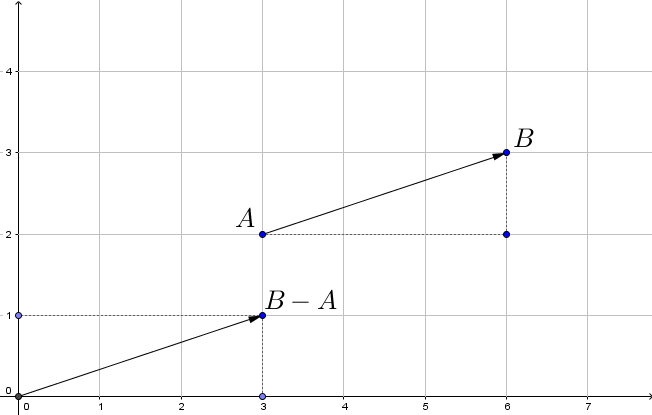
\includegraphics[width=0.6\linewidth]{img/vettori_1.png}	
\end{center}

\begin{align*}
	A(3,3) \qquad B(6,4) \\
	B-A=(6-3,4-3)=(3,1) = B + (-A)
\end{align*}
\subsection{Prodotto scalare}
Il prodotto scalare di due vettori A e B si indica con $A\cdot B$, ed è un elemento del campo numerico dello spazio vettoriale.\\\\
\textbf{Esempio}\\
\begin{gather*}
	A(a_1,a_2)\\
	B(b_1,b_2)\\
	A\cdot B = a_1\cdot b_1 + a_2\cdot b_2
\end{gather*}
Il prodotto scalare di un vettore per se stesso è uguale al quadrato del modulo: $A\cdot A = ||A||^2 = a^2 + b^2$, dove $a$ e $b$ sono i coefficienti di $x$ e $y$.

\pagebreak
\subsection{Operazioni vettoriali}
Dati dei vettori $A=(a_1, a_2, a_3)$ e $B=(b_1, b_2, b_3)$
\begin{gather*}
	A\cdot B = a_1b_1 + a_2b_2 + a_3b_3\\
	||A||\cdot ||B|| \cdot cos(\alpha) = A\cdot B
\end{gather*}
Il punto A è inteso come punto del piano o dello spazio.\\
I vettori godono delle seguenti proprietà:
\begin{itemize}
	\item proprietà commutativa:  $A\cdot B = B\cdot A$
	\item proprietà distributiva: $A\cdot (B+C) = A\cdot B + A \cdot C$
\end{itemize}
Esempi proprietà:
\begin{itemize}
	\item proprietà commutativa:  $a_1b_1 + a_2b_2 + a_3b_3 = b_1a_1 + b_2a_2 + b_3a_3$
	\item proprietà distributiva: $a_1(b_1+c_1)+a_2(b_2c_2) + a_3(b_3c_3) = a_1b_1 + a_1c_1 + a_2b_2 + a2_c2+a_3b_3+a_3c_3$
\end{itemize}
\subsubsection{Prodotto scalare}

La lunghezza di un vettore è definita come
\[
	||A|| = A\cdot A \to \text{[A prodotto interno A]}
\]\\
$\vec{0}\cdot \vec{0} = 0$ \qquad \textit{[vettore 0 moltiplicato vettore 0 = numero 0]}\\\\
Il prodotto scalare \textbf{può essere negativo}, mentre il prodotto scalare di un vettore per se stesso è uguale al quadrato del modulo.\\\\
Quando ottengo il prodotto scalare 0 significa che il coseno è 0, quindi i \textbf{due vettori} sono \textbf{perpendicolari}.

\subsubsection{Dimostrazione teorema}

\[(A\cdot B)^2 \leq (A\cdot A)(B\cdot B)\]
\begin{gather*}
	(A\cdot B)^2 \leq ||A||^2 \cdot ||B||^2 \qquad \emph{[sempre positivo]} \\
	(A\cdot B) \leq ||A|| \cdot ||B|| \qquad \emph{[può essere negativo, aggiungo il modulo a sinistra (a destra c'è già)]} \\
	|A\cdot B| \leq ||A|| \cdot ||B|| \\
\end{gather*}
\begin{gather*}
	A=(1,3,-2) \qquad ||A||=\sqrt{1^2+3^2+(-2)^2}=\sqrt{14} \\
	B=(-1,4,3) \qquad ||B|| = \sqrt{(-1)^2+4^2+3^2}=\sqrt{26}
\end{gather*}
\begin{gather*}
	|A\cdot B| \leq ||A||\cdot||B|| \\
	5 \leq \sqrt{14} \cdot \sqrt{26} \\
	5^2 \leq 14\cdot 26 \\
	25 \leq 364
\end{gather*}


\pagebreak
\subsection{Vettori perpendicolari}
Distanza tra due punti nel piano: $\sqrt{(b_1-a_1)^2+(b_2-a_2)}$\\\\
$A\cdot B = 0$ sse i vettori sono perpendicolari.\\\\
Due vettori sono perpendicolari quando (dimostrazione):
\begin{gather*}
	||A-B||=||A-(-B)||\rightarrow||A-B||=||A+B|| \\
	(A-B)\cdot (A-B)=(A+B)(A+B) \\
	\cancel{A^2}-2AB+\cancel{B^2} = \cancel{A^2}+2AB+\cancel{B^2} \rightarrow 4AB=0 \to AB=0
\end{gather*}




Il prodotto scalare è negativo quando l'angolo è > di $\frac{\pi}{3}$\\\\
\underline{The other shit goes here...}

\pagebreak
\section{Altri vettori}

\subsection{Rette parallele e perpendicolari}
Esempio 1
\begin{center}
	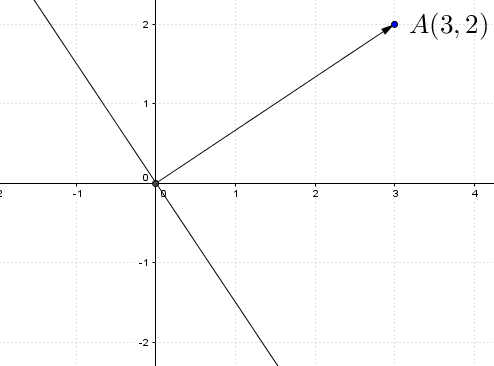
\includegraphics[width=0.5\linewidth]{img/vettori_rette_0.png} 
\end{center}
Esempio 2
\begin{center} 
	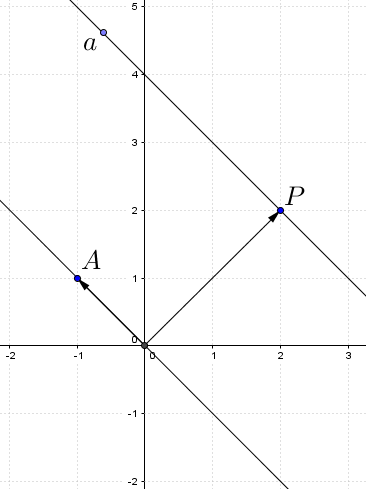
\includegraphics[width=0.4\linewidth]{img/vettori_rette_1.png}
\end{center}
\pagebreak
\subsubsection{Rappresentazioni alternative}
I vettori si possono rappresentare come punti nel piano, delimitati dal punto e dal segmento che va dall'origine degli assi al punto stesso.


\begin{gather*}
	3x+2y=0 \emph{[è un'equazione lineare]}
\end{gather*}
Posso scriverlo come: 
\begin{gather*}
	(3,2)\cdot(x,y)=0
\end{gather*}


Un altro modo è trasformare un'equazione in un altra equazione, ma parametrica:
\begin{gather*}
	R=\{(x,y):3x+2y=0\}
\end{gather*}


Il punto $(2,-3)$  sta nella retta.
Una volta che scoperto che il punto è sulla retta, se moltiplico la coppia per lo scalare t, al variare di \emph{t} ottengo tutti i punti (\textit{vettori}) che stanno sulla stessa retta.
\subsubsection{Esempio}
\begin{gather*}
	\begin{split}
		3x+2y=5 &\to (3,2)\cdot (x,y) = 5\\
		&\to \sqrt{13}\cdot \sqrt{x^2+y^2}\cdot \cos(\alpha)
	\end{split}\\
	\sqrt{x^2+y^2}\cdot \cos(\alpha) = \frac{5}{\sqrt{13}} \qquad \emph{[dobbiamo capire che retta è]}\\
\end{gather*}
Risolvo l'equazione e scopro che $(1,1)$ appartiene alla retta:

\begin{enumerate}[label=$\rightarrow$]
	\item $t(2,-3)=(2t,-3t) \rightarrow x'=1+2t, x=2t, y'=1-3t, y=-3t$ 
	\item $(1,1)+(2,-3)=(3,-2) \rightarrow 3\cdot 3 + 2\cdot (-2) = 9 - 4 =  5$ 
	\item $3\cdot (1+2) + 2\cdot (1-3) = 5$ 
	\item $x=\frac{3}{2}-2t$
\end{enumerate}

\pagebreak
\section{Sistemi lineari}
Un sistema di equazioni lineari, anche detto sistema lineare, è un sistema di equazioni lineari che devono essere verificate tutte contemporaneamente. Una soluzione del sistema è un vettore i cui elementi sono le soluzioni delle equazioni che compongono il sistema, ovvero tali che se sostituiti alle incognite rendono le equazioni delle identità.

\begin{gather*}
	3x + 5y + z = 7 \\
	\begin{cases*}
		(3,5,1)(x,y,z)=7\\
		(3,5,1)(x,y,z)=0
	\end{cases*}
	\to \text{sono due vettori diversi, ma paralleli ($A \parallele B$)} 
\end{gather*}
Nello spazio vettoriale, se abbiamo 3 punti non allineati \textit{(quindi non sullo stesso piano)}, vi sarà un piano che li attraversa.\\\\
\textbf{Numero di possibili soluzioni} in generale. Il sistema ammette
un’unica soluzione se le due rette non sono parallele e quindi si intersecano. Se le rette sono parallele, allora non abbiamo soluzioni, mentre abbiamo infinite soluzioni se le due rette coincidono.\\\\
Per \underline{determinare il numero di soluzioni} di un sistema lineare, dobbiamo calcolare il \underline{prodotto interno} di A e B.\\\\
\textbf{Esempio}
\begin{gather*}
	\begin{cases*}
		(3,2)(x,y)=5\\
		(1,4)(x,y)=3
	\end{cases*}	
	\to \text{sono parallele?}\\
	A\cdot B = (3,2)(1,4)=3\cdot 1 + 2 \cdot 4 = 11
\end{gather*}
Trovati $||A|| = \sqrt{13}$ e $||B|| = \sqrt{17}$, determiniamo il coseno dell'angolo tra i due vettori
\begin{gather*}
	\cos (\theta) = \dfrac{A\cdot B}{||A||\cdot ||B||}\\\\
	\cos (\theta) = \dfrac{11}{\sqrt{13}\cdot \sqrt{17}} = \sqrt{\dfrac{212}{221}} < 1	\to \text{i due vettori non sono paralleli}
\end{gather*}
Due vettori sono paralleli quando $\cos (\theta) = 1 $ oppure $\cos (\theta) = -1 $\\\\
\textbf{Esempio}
\begin{gather*}
	\begin{cases*}
		3x+2y+z=5\\
		x+4y+3z=3\\
		x+y+z = 0
	\end{cases*}	
	\to \text{come determiniamo il numero di soluzioni?}\\\\
	A(3,2,1)\\
	B(1,4,3)\\
	C(1,1,1)\\\\
	A\cdot B = 14\\
	A \cdot C = 6\\
	B\cdot C = 8
\end{gather*}
\[
	\left.
	\begin{aligned}
		\cos (\theta)_{AB} = \dfrac{14}{\sqrt{14}\cdot \sqrt{26}} < 1 \\
		\cos (\theta)_{AC} = \dfrac{6}{\sqrt{14}\cdot \sqrt{3}}  < 1  \\
		\cos (\theta)_{BC} = \dfrac{8}{\sqrt{26}\cdot \sqrt{3}}  < 1
	\end{aligned}
	\right\rbrace \to \text{1 unica soluzione}
\]
\pagebreak\\
\textbf{Esempio}\\
\begin{gather*}
	\begin{cases*}
		x+2y+3z=4\\
		5x+2y+6z=7\\
		-x+y-z=1
	\end{cases*}\\\\
	A = (1,2,3)\\
	B = (5,2,6)\\
	C = (-1,1,-1)\\\\
	A\cdot B = 1\cdot 5 + 2\cdot 2 + 3 \cdot 6 = 27\\
	A\cdot C = 1\cdot (-1) + 2\cdot 1 + 3 \cdot (-1) = -2\\
	B\cdot C = 5\cdot (-1) + 2\cdot 1 + 6 \cdot (-1) = -9\\\\
	||A|| = \sqrt{1^2 + 2^2 + 6^2} = \sqrt{14}\\
	||B|| = \sqrt{5^2 + 2^2 + 6^2} = \sqrt{65}\\
	||C|| = \sqrt{(-1)^2+1^2+(-1)^2} = \sqrt{3}\\\\
	\left.
		\begin{aligned}
			\cos (\theta)_{AB} = \frac{27}{\sqrt{14}\cdot \sqrt{65}} < 1 \\
			\cos (\theta)_{AC} = \frac{-2}{\sqrt{14}\cdot \sqrt{3}}  < 1  \\
			\cos (\theta)_{BC} = \frac{-9}{\sqrt{65}\cdot \sqrt{3}}  < 1
		\end{aligned}
	\right\rbrace \to \text{1 unica soluzione}
\end{gather*}
Inizio risoluzione del sistema
\begin{gather*}
	\begin{cases*}
		x+2y+3z=4 \qquad \text{moltiplico tutto per 5 per far coincidere i coefficienti di x} \\
		5x+2y+6z=7\\
		-x+y-z=1
	\end{cases*}\\\\
	5x + 10y + 15z=20 \qquad \text{dato da 5 $\times$ prima riga}\\
	0x -8y -9z = -13 \qquad \text{sottraggo la prima riga dalla seconda [\textit{combinazione lineare}]}\\\\
	\begin{cases*}
		x+2y+3z=4\\
		-8y-9z=-13 \qquad \text{sostituisco con la combinazione lineare appena trovata}\\
		-x+y-z=1
	\end{cases*}\\\\
	+x+2y+3z=4 \quad +\\
	-x + y -1z=1 \quad =\\
	0x + 3y + 2z =5 \qquad \text{sommo (o sottraggo) la seconda riga dalla terza}\\\\
	\begin{cases*}
		x+2y +3z=4\\
		-8y-9z=-13\\
		3y+2z=5
	\end{cases*}\\\\
	\frac{3}{8}\cdot (-8y-9z)=\frac{3}{8}\cdot (-13) \qquad \text{voglio che il coefficiente della $y$ sia uguale a 3}\\
	= -3y -\frac{27}{8}z = -\frac{39}{8}\\\\
	3y+2z=5 \quad + \\
	-3y -\frac{27}{8}z = -\frac{39}{8} \\ 
	= \to -\frac{11}{8}z = \frac{1}{8}\\\\
	\begin{cases*}
		x+2y+3z=4\\
		-8y-9z=-13\\
		-\frac{11}{8}y=\frac{1}{8}
	\end{cases*}
	\qquad
	\begin{cases*}
		x = \frac{9}{11}\\
		y = \frac{19}{11} \\
		z=-\frac{1}{11}
	\end{cases*}
\end{gather*}
Ora verifico che i risultati ottenuti di $x,y,z$ soddisfino il sistema iniziale:
\begin{gather*}
	(1) \qquad \frac{9}{11} + 2\cdot \frac{19}{11} - \frac{3}{11} = 4 \Rightarrow \frac{9}{11} + \frac{38}{11} - \frac{3}{11} \Rightarrow \frac{44}{11} = 4 \Rightarrow 4=4  \text{ vero}\\
	(2) \qquad 5\cdot \frac{9}{11} + 2\cdot \frac{19}{11} - \frac{6}{11} = 7 \Rightarrow \frac{45}{11} + \frac{38}{11} - \frac{6}{11} \Rightarrow \frac{77}{11} = 7 \Rightarrow 7=7  \text{ vero}\\
	(3) \qquad -\frac{9}{11} + \frac{19}{11} + \frac{1}{11} = 1 \Rightarrow \frac{11}{11} = 1 \Rightarrow 1=1  \text{ vero}\\
\end{gather*}
Il sistema è stato verificato.
\pagebreak\\
\subsection{Sistemi lineari e matrici}
\begin{gather*}
	\begin{cases*}
		3x+2y+z=5\\
		x+4y+3z=3
	\end{cases*}
\end{gather*}
Se i piani sono paralleli sono vi sono soluzioni, se sono sovrapposti vi sono infinite soluzioni mentre se si incrociano vi è una retta di soluzioni.
\begin{gather*}
		A = (3,2,1)\\
		B = (1,4,3)\\\\
		||A|| = \sqrt{3^2 + 2^2 + 1^2} = \sqrt{14}\\
		||B|| = \sqrt{1^2 + 4^2 + 3^2} = \sqrt{26}\\\\
		A\cdot B = 3\cdot 1 + 2\cdot 4 + 1 \cdot 3 = 14\\\\
		\cos (\theta)_{AB} = \frac{14}{\sqrt{14}\cdot \sqrt{26}} < 1 \to \text{la soluzione è una retta}\\\\
		3\cdot(x+4y+3z)=3\cdot 3 \qquad \text{moltiplico la seconda riga per 3, per far combaciare i coefficienti delle $x$}\\
		\Rightarrow 3x + 12y +9z = 9\\\\
		3x+12y+9z=9 \qquad +\\
		-3x - 2y - z = -5 \quad \Rightarrow \quad 10y+8z=4 \quad \Rightarrow \quad 5y+4z=2\\\\
		\begin{cases*}
			3x+2y+z=5\\
			5y+4z=2
		\end{cases*}
		\qquad
		\begin{cases*}
			3x=-2y-z+5\\
			5y=2-4z
		\end{cases*}
		\qquad
		\begin{cases*}
			3x=-2y-z+5\\
			y=\frac{2}{5}-\frac{4}{5}z
		\end{cases*}
		\qquad
		\begin{cases*}
			3x=-2(\frac{2}{5}-\frac{4}{5}z)-z+5\\
			y=\frac{2}{5}-\frac{4}{5}z
		\end{cases*}
		\\\\
		\begin{cases*}
			3x=-\frac{4}{5} + \frac{8}{5}z-z+5\\
			y=\frac{2}{5}-\frac{4}{5}z
		\end{cases*}
		\qquad
		\begin{cases*}
			x=\frac{21}{5} - \frac{3}{5}z-z+5\\
			y=\frac{2}{5}-\frac{4}{5}z
		\end{cases*}
\end{gather*}\\
Matrici dei coefficienti:
\[
	\begin{bmatrix}
		3 & 2 & 1 \\
		1 & 4 & 3
	\end{bmatrix}
\]
Matrice dei coefficienti con i punti:
\[
	\begin{bmatrix}
		3 & 2 & 1 & 5\\
		1 & 4 & 3 & 3
	\end{bmatrix}
\]\\
Sia $\mathbb{D}$ un campo numerico. Una matrice $A=(A_{ij})$ con $m$ righe e $n$ colonne, è una famiglia di $m\times n$ elementi del campo.
\pagebreak
\section{Matrici}
Una matrice $A$ è quadrata se $m=n$, ovvero quando le righe sono tante quante le colonne:
\[
\begin{bmatrix} 
	a_{11} & \cdots & a_{1n} \\
	\vdots & \ddots & \vdots \\
	 a_{n1} & \cdots & a_{mn}
\end{bmatrix}
\]
Una matrice \textbf{quadrata} $A$ è simmetrica se $A_{ij} = A_{ji}$
\[
	\begin{bmatrix} 
		\textcolor{red}{1} & \textcolor{blue}{2} & \textcolor{ForestGreen}{3} \\
		\textcolor{blue}{2} & \textcolor{red}{1} & 4 \\
		\textcolor{ForestGreen}{3} & 4 & \textcolor{red}{1}
	\end{bmatrix}
\]
Una matrice \textbf{quadrata} $A$ è \textbf{diagonale} se $A_{ij} = 0$ per $i\neq j$
\[
	\begin{bmatrix} 
		\textcolor{red}{2} & 0 & 0 \\
		0 & \textcolor{red}{1} & 0 \\
		0 & 0 & \textcolor{red}{3}
	\end{bmatrix}
\]
Una matrice $A$ è \textbf{triangolare} \textbf{superiore} se $A_{ij} = 0$ per $i > 0$
\[
	\begin{bmatrix} 
		1 & 3 & 4 \\
		\textcolor{red}{0} & 6 & 1 \\
		\textcolor{red}{0} & \textcolor{red}{0} & 7
	\end{bmatrix}
\]\\\\
Sia $A$ una matrice $m\times n$. Allora la \textbf{trasposta} di $A$ si indica con $A^T$, ed è una matrice $n\times m$, e $A^T_{ij} = A_{ji}$
\begin{gather*}
	A = 
	\begin{bmatrix} 
		\textcolor{red}{3} & \textcolor{red}{2} & \textcolor{red}{1} & \textcolor{red}{0} \\
		1 & 2 & 2 & 3 \\
		4 & 5 & 6 & 7
	\end{bmatrix}\\\\	
	A^T =
	\begin{bmatrix} 
		\textcolor{red}{3} & 1 & 4 \\
		\textcolor{red}{2} & 2 & 5 \\
		\textcolor{red}{1} & 2 & 6 \\
		\textcolor{red}{0} & 3 & 7
	\end{bmatrix}\\\\
	(A^T)^T = A
\end{gather*}\\
Siano $A$ e $B$ due matrici $m\times n$:
\begin{gather*}
	A = 
	\begin{bmatrix} 
		5 & 4 & 3 \\
		1 & 2 & 3 \\
		4 & 6 & 1
	\end{bmatrix}\\\\
	B = 
	\begin{bmatrix} 
		7 & 9 & 1 \\
		4 & 0 & 2 \\
		5 & 0 & 5
	\end{bmatrix}\\\\
	A+B =
	\begin{bmatrix} 
		5 & 4 & 3 \\
		1 & 2 & 3 \\
		4 & 6 & \textcolor{red}{1}
	\end{bmatrix}
	+
	\begin{bmatrix} 
		7 & 9 & 1 \\
		4 & 0 & 2 \\
		5 & 0 & \textcolor{red}{5}
	\end{bmatrix}
	=
	\begin{bmatrix} 
		12 & 13 & 4 \\
		5 & 2 & 5 \\
		9 & 6 & \textcolor{red}{6}
	\end{bmatrix}\\\\
	5\cdot A =
	5\cdot 
	\begin{bmatrix} 
	5 & 4 & 3 \\
	1 & 2 & 3 \\
	4 & 6 & 1
	\end{bmatrix}
	=
	\begin{bmatrix} 
	25 & 20 & 15 \\
	5 & 10 & 15 \\
	20 & 30 & 5
	\end{bmatrix}
\end{gather*}
L'insieme di tutte le matrici  $m\times n$ sul campo $\mathbb{K}$ è uno spazio vettoriale con la somma (matriciale) componente per componente e prodotto scalare. 

\pagebreak
\subsection{Esercizio 1}
\begin{gather*}
	\begin{cases*}
		3x+2y=5\\
		x+
		y=0
	\end{cases*}
\end{gather*}
Per risolvere il sistema, possiamo creare la matrice dei coefficienti e ricavarci una matrice triangolare superiore.\\\\
Matrice dei coefficienti:
\begin{gather*}
	\begin{bmatrix}
		3 & 2 \\
		1 & 7
	\end{bmatrix}
	\cdot
	\begin{bmatrix}
		x \\ y
	\end{bmatrix}
	=
	\begin{bmatrix}
		5 \\ 0
	\end{bmatrix}
\end{gather*}
Costruzione matrice triangolare superiore:
\begin{gather*}
	\begin{bmatrix}
		3 & 2 & 5 \\
		1 & 7 & 0
	\end{bmatrix}
	\to \text{moltiplico la prima riga per $-\nicefrac{1}{3}$ e la sottraggo dalla seconda}\\
	\begin{bmatrix}
		3 & 2 & 5 \\
		1 -(\nicefrac{1}{3} \cdot 3) & 7 -(\nicefrac{1}{3} \cdot 2) & 0 -(\nicefrac{1}{3} \cdot 5)
	\end{bmatrix}
	=
	\begin{bmatrix}
		3 & 2 & 5 \\
		0 & \nicefrac{2}{3} & -\nicefrac{5}{3}
	\end{bmatrix}
\end{gather*}
\subsection{Prodotto matriciale}
Se abbiamo una matrice $A$ di dimensione $\textcolor{red}{m} \times n$ e una matrice $B$ di dimensione $n \times \textcolor{red}{k}$ allora possiamo definire il prodotto matriciale $A\cdot B$ di dimensione $\textcolor{red}{m} \times \textcolor{red}{k}$.\\\\
Esempio:
\begin{gather*}
	\begin{bmatrix}
		3 & 2 & 5 \\
		1 & 7 & 0
	\end{bmatrix}
	\cdot
	\begin{bmatrix}
		1 & 2 \\
		3 & 4 \\
		5 & 6
	\end{bmatrix}
	=
	\begin{bmatrix}
		3\cdot 1 + 2 \cdot 3 + 5 \cdot 5 & 3\cdot 2 + 2 \cdot 4 + 5 \cdot 6 \\
		1\cdot 1 + 7 \cdot 3 + 0 \cdot 5 & 1\cdot 2 + 7 \cdot 4 + 0 \cdot 6
	\end{bmatrix}
	=
	\begin{bmatrix}
		34 & 44 \\
		22 & 30
	\end{bmatrix}
\end{gather*}

\subsection{Proprietà delle matrici}
\begin{itemize}
	\item $A(BC) = (AB)$
	\item identità: $AI = IA = A$
	\item nulla: $0A = A0 = 0$
	\item $A(B+C) = AB + AC$
	\item $(B+C)A = BA + CA$
	\item $AA^{-1} = A^{-1}A = I$
\end{itemize}
\pagebreak
\textbf{Dimensioni matrice di un prodotto}:
\begin{gather*}
	A =
	\begin{bmatrix}
		1 & 2 \\
		3 & 4
	\end{bmatrix}
	\qquad \Rightarrow  2\times2\\
	B =
	\begin{bmatrix}
		3 & 2 & 5 \\
		2 & -2 & 4
	\end{bmatrix}
	\qquad \Rightarrow 2\times3 \\
	C =
	\begin{bmatrix}
		1 & -2 & 1 \\
		-4 & -2 & 1 \\
		2 & -2 & 3
	\end{bmatrix}
	\qquad \Rightarrow 3\times3 \\
	A\cdot B = (\textcolor{red}{2}\times2) \cdot (2\times\textcolor{red}{3}) = (\textcolor{red}{2}\times\textcolor{red}{3})\\
	A\cdot B\cdot C = (A\cdot B)\cdot C = (\textcolor{red}{2}\times3)\cdot(3\times\textcolor{red}{3}) = (\textcolor{red}{2}\times\textcolor{red}{3})
\end{gather*}
\textbf{Esempio prodotto matriciale}\\
\begin{gather*}
	A = 
	\begin{bmatrix}
		1 & 2 \\
		3 & 4
	\end{bmatrix} \qquad \Rightarrow 2 \times 2 \\
	B =
	\begin{bmatrix}
		3 & 2 & 5 \\
		2 & -2 & 4
	\end{bmatrix} \qquad \Rightarrow 3 \times 2 \\
	C = 
	\begin{bmatrix}
		1 & -2 & 1 \\
		-4 & -2 & 1 \\
		2 & -2 & 3
	\end{bmatrix} \qquad \Rightarrow 3 \times 3 \\\\
	A\cdot B \cdot C = 
	\begin{bmatrix}
		1 & 2 \\
		3 & 4
	\end{bmatrix}
	\cdot
	\begin{bmatrix}
		3 & 2 & 5 \\
		2 & -2 & 4
	\end{bmatrix}
	\cdot
	\begin{bmatrix}
		1 & -2 & 1 \\
		-4 & -2 & 1 \\
		2 & -2 & 3
	\end{bmatrix}\\\\
	A\cdot B =
	\begin{bmatrix}
		1 & 2 \\
		3 & 4
	\end{bmatrix}
	\cdot
	\begin{bmatrix}
		3 & 2 & 5 \\
		2 & -2 & 4
	\end{bmatrix}
	=
	\begin{bmatrix}
		7 & -2 & 13 \\
		17 & -2 & 31
	\end{bmatrix}\\\\
	A\cdot B \cdot C =
	\begin{bmatrix}
		7 & -2 & 13 \\
		17 & -2 & 31
	\end{bmatrix}
	\cdot
	\begin{bmatrix}
		1 & -2 & 1 \\
		-4 & -2 & 1 \\
		2 & -2 & 3
	\end{bmatrix}
	=
	\begin{bmatrix}
		41 & -36 & 44 \\
		87 & -92 & 108
	\end{bmatrix}
\end{gather*}\\

\pagebreak
\subsection{Esercizio} 
Data una matrice, ricavarne una triangolare superiore
\begin{gather*}
	\text{Origine}\\
	\begin{bmatrix}
		1 & 1 & 1 & 0 \\
		3 & 2 & 1 & 5 \\
		1 & 4 & 3 & 3
	\end{bmatrix}
	\\\\
	\text{\textbf{a.} Sottraggo 3 volte la prima riga dalla seconda}\\
	\begin{bmatrix}
		1 & 0 & 0 \\
		\textcolor{red}{-3} & 1 & 0 \\
		0 & 0 & 1
	\end{bmatrix}
	\\\\
	\text{\textbf{b.} Sottraggo la prima riga dalla terza}\\
	\begin{bmatrix}
		1 & 0 & 0 \\
		0 & 1 & 0 \\
		\textcolor{red}{-1} & 0 & 1
	\end{bmatrix}
	\\\\
	\text{\textbf{c.} Sommo 3 volte la seconda riga alla terza}\\
	\begin{bmatrix}
		1 & 0 & 0 \\
		0 & 1 & 0 \\
		0 & \textcolor{red}{3} & 1
	\end{bmatrix}
	\\\\
	\text{Se ora moltiplico ogni punto per la matrice di origine, ottengo la matrice triangolare superiore}
	\\\\
	\text{Origine moltiplicata per a}
	\begin{bmatrix}
		1 & 1 & 1 & 0 \\
		3 & 2 & 1 & 5 \\
		1 & 4 & 3 & 3
	\end{bmatrix}
	\cdot
	\begin{bmatrix}
		1 & 0 & 0 \\
		-3 & 1 & 0 \\
		0 & 0 & 1
	\end{bmatrix}
	=
	\begin{bmatrix}
		1 & 1 & 1 & 0 \\
		\textcolor{red}{0} & -1 & -2 & 5 \\
		1 & 4 & 3 & 3
	\end{bmatrix}
	\\\\
	\text{Risultato moltiplicato per b}
	\begin{bmatrix}
		1 & 1 & 1 & 0 \\
		\textcolor{red}{0} & -1 & -2 & 5 \\
		1 & 4 & 3 & 3
	\end{bmatrix}
	\cdot
	\begin{bmatrix}
		1 & 0 & 0 \\
		0 & 1 & 0 \\
		-1 & 0 & 1
	\end{bmatrix}
	=
	\begin{bmatrix}
		1 & 1 & 1 & 0 \\
		\textcolor{red}{0} & -1 & -2 & 5 \\
		\textcolor{red}{0} & 4 & 3 & 3
	\end{bmatrix}
	\\\\
	\text{Risultato moltiplicato per c}
	\begin{bmatrix}
		1 & 1 & 1 & 0 \\
		\textcolor{red}{0} & -1 & -2 & 5 \\
		\textcolor{red}{0} & 4 & 3 & 3
	\end{bmatrix}
	\cdot
	\begin{bmatrix}
		1 & 0 & 0 \\
		0 & 1 & 0 \\
		0 & 3 & 1
	\end{bmatrix}
	=
	\begin{bmatrix}
	1 & 1 & 1 & 0 \\
	\textcolor{red}{0} & -1 & -2 & 5 \\
	\textcolor{red}{0} & \textcolor{red}{0} & 3 & 3
	\end{bmatrix}
\end{gather*}

\pagebreak
\subsection{Esercizio} Scambiare la prima riga con la terza
\begin{gather*}
	\begin{bmatrix}
		0 & 0 & 1 \qquad \text{3\textdegree \;riga}\\
		0 & 1 & 0 \qquad \text{2\textdegree \;riga}\\
		1 & 0 & 0 \qquad \text{1\textdegree \;riga}
	\end{bmatrix}
	\Rightarrow 
	\text{Quando moltiplico una matrice per questa, la prima riga e la terza sono scambiate}
\end{gather*}
\subsection{Esercizio} Sommare alla seconda riga 100 volte la prima
\begin{gather*}
	\begin{bmatrix}
		1 & 0 & 0 \\
		100 & 1 & 0 \\
		0 & 0 & 1 
	\end{bmatrix}
	\Rightarrow 
	\text{Quando moltiplico una matrice per questa, la prima riga è sommata 100 volte alla seconda}
\end{gather*}
\subsection{Esercizio} Sommare alla terza riga 50 volte la prima riga e 3 volte la seconda
\begin{gather*}
	\begin{bmatrix}
		1 & 0 & 0 \\
		0 & 1 & 0 \\
		50 & 3 & 1 
	\end{bmatrix}
\end{gather*}

\subsection{Esericizio}
Risolvere un sistema lineare con le matrici
\[
	\begin{bmatrix}
		1 & 5 & -2 \\
		3 & 0 & -6 \\
		-2 & 1 & 3
	\end{bmatrix}
	\cdot
	\begin{bmatrix}
		x_1 \\ x_2 \\ x_3
	\end{bmatrix}
	=
	\begin{bmatrix}
		1 \\ 1 \\ 1
	\end{bmatrix}
\]
Devo ottenere una matrice triangolare superiore, quindi
\begin{enumerate}[label=\alph*.]
	\item Sottraggo 3 volte la prima riga alla seconda
	\item Sommo due volte la prima riga alla terza
\end{enumerate}
\[
	\begin{bmatrix}
		1 & 0 & 0 \\
		-3 & 1 & 0 \\
		2 & 0 & 1
	\end{bmatrix}
	\cdot
	\begin{bmatrix}
		1 & 5 & -2 & 1\\
		3 & 0 & -6 & 1\\
		-2 & 1 & 3 & 1 
	\end{bmatrix}
	=
	\begin{bmatrix}
		1 & 5 & -2 & 1\\
		0 & -15 & 0 & -2\\
		0 & 11 & -1 & 3 
	\end{bmatrix}
\]
Ora devo rendere $0$ anche il valore in posizione $[3,2]$, ovvero il numero $11$. \\Per farlo dovrò moltiplicare la seconda riga per $\nicefrac{11}{15}$ e infine sottrarla alla terza riga
\[
	\begin{bmatrix}
		1 & 0 & 0 \\
		0 & 1 & 0 \\
		0 & \nicefrac{11}{15} & 1
	\end{bmatrix}
	\cdot
	\begin{bmatrix}
		1 & 5 & -2 & 1\\
		0 & -15 & 0 & -2\\
		0 & 11 & -1 & 3 
	\end{bmatrix}
	=
	\begin{bmatrix}
		1 & 5 & -2 & 1 \\
		0 & -15 & 0 & -2 \\
		0 & 0 & -1 & \nicefrac{23}{11}
	\end{bmatrix}
\]
Ora verifico che il risultato ottenuto sia corretto
\[
	\begin{bmatrix}
		1 & 0 & 0 \\
		0 & 1 & 0 \\
		0 & \nicefrac{11}{15} & 1
	\end{bmatrix}
	\cdot
	\begin{bmatrix}
		1 & 0 & 0 \\
		-3 & 1 & 0 \\
		2 & 0 & 1
	\end{bmatrix}
	=
	\begin{bmatrix}
		1 & 0 & 0 \\
		-3 & 1 & 0 \\
		-\nicefrac{1}{5} & \nicefrac{11}{15} & 1
	\end{bmatrix}
	\Rightarrow
	\begin{bmatrix}
		1 & 0 & 0 \\
		-3 & 1 & 0 \\
		-\nicefrac{1}{5} & \nicefrac{11}{15} & 1
	\end{bmatrix}
	\cdot
	\begin{bmatrix}
		1 & 5 & -2 & 1\\
		0 & -15 & 0 & -2\\
		0 & 11 & -1 & 3 
	\end{bmatrix}
	=
	\begin{bmatrix}
		1 & 5 & -2 & 1 \\
		0 & -15 & 0 & -2 \\
		0 & 0 & -1 & \nicefrac{23}{11}
	\end{bmatrix}
\]
Corretto

\pagebreak
\section{Matrici inverse}
\subsection{Esercizio}
Trovare la matrice inversa.\\\\
\textit{La matrice si dice inversa quando se moltiplicata per la matrice di origine ottengo la matrice identica}\\
\[
	\begin{bmatrix}
		1 & 0 & 0 \\
		x & 1 & 0 \\
		0 & 0 & 1
	\end{bmatrix}
	\xrightarrow{\text{inversa}}
	\begin{bmatrix}
		1 & 0 & 0 \\
		-x & 1 & 0 \\
		0 & 0 & 1
	\end{bmatrix}
\]
Infatti se moltiplico queste due matrici ottengo:
\[
	\begin{bmatrix}
		1 & 0 & 0 \\
		x & 1 & 0 \\
		0 & 0 & 1
	\end{bmatrix}
	\cdot
	\begin{bmatrix}
		1 & 0 & 0 \\
		-x & 1 & 0 \\
		0 & 0 & 1
	\end{bmatrix}
	=
	\begin{bmatrix}
		1 & 0 & 0 \\
		0 & 1 & 0 \\
		0 & 0 & 1
	\end{bmatrix}
\]
La prima matrice, infatti, significa "\textit{sommo x volte la prima riga alla seconda}", mentre l'inversa "\textit{sottraggo x volte la prima riga dalla seconda}".

\subsection{Determinante di una matrice}
Data una matrice
\[
	A =
	\begin{bmatrix}
		a & b \\
		c & d
	\end{bmatrix}
	\qquad
	B =
	\begin{bmatrix}
		1 & 2 \\
		3 & 4
	\end{bmatrix}
\]
Il determinante della matrice $A$ si calcola come 
\[
	det(A) = a\cdot d - b \cdot c
\]
Se ad esempio devo trovare il determinante di B:
\[
	det(B) = 1 \cdot 4 - 2 \cdot 3 = -2
\]
Se il determinante è diverso da zero la matrice è invertibile, quindi se
\[
	\text{se } det(A) = 0 \quad \text{la matrice \textbf{non} è invertibile}
\]
Il determinante di una matrice è $0$ solo quanto le due rette della soluzione (se quadrata) sono parallele o coincidenti.
\subsection{Matrice inversa}
Per trovare la matrice inversa posso
\[
	A^{-1} = \frac{1}{det(A)} \cdot
	\begin{bmatrix}
		d & -b \\
		-c & a
	\end{bmatrix}
\]
per verificare che sia veramente la matrice inversa, faccio la controprova:
\begin{gather*}
	\begin{split}
		\begin{bmatrix}
			a & b \\
			c & d
		\end{bmatrix}
		\cdot
		\left(
			\frac{1}{det(A)} \cdot
			\begin{bmatrix}
				d & -b \\
				-c & a
			\end{bmatrix}
		\right) &= \\
		&= 
		\frac{1}{det(A)} \cdot
		\begin{bmatrix}
			ad-bc & a(-b) + ba = 0\\
			a(-b) + ba = 0 & ad-bc
		\end{bmatrix}\\
		&=
		\frac{1}{det(A)} \cdot
		\begin{bmatrix}
		ad-bc & 0\\
		0 & ad-bc
		\end{bmatrix}\\
		&=
		\begin{bmatrix}
			1 & 0 \\
			0 & 1
		\end{bmatrix}
	\end{split}
\end{gather*}

\newpage
\subsection{Matrice inversa - metodo 1}
Calcolare la matrice inversa di
\[
	B =
	\begin{bmatrix}
		1 & 2 \\
		3 & 4
	\end{bmatrix}
\]
Calcolo il determinante
\[
	det(B) = 1 \cdot 4 - 2 \cdot 3 = -2
\]
Inverto la diagonale della matrice e cambio segno sulla diagonale opposta
\[
	B =
	\begin{bmatrix}
		1 & 2 \\
		3 & 4
	\end{bmatrix}
	\Rightarrow
	\begin{bmatrix}
		4 & -2 \\
		-3 & 1
	\end{bmatrix}
\]
Ora divido ogni termine della matrice per il determinante
\[
	-\frac{1}{2} \cdot
	\begin{bmatrix}
		4 & -2 \\
		-3 & 1
	\end{bmatrix}
	=
	\begin{bmatrix}
		\frac{4}{-2} & \frac{-2}{-2} \\[3mm]
		\frac{-3}{-2} & \frac{1}{-2}
	\end{bmatrix}
	=
	\begin{bmatrix}
		-2 & 1 \\[1mm]
		\frac{3}{2} & -\frac{1}{2}
	\end{bmatrix}
\]
verifico che la matrice sia veramente l'inversa
\[
	\begin{bmatrix}
		1 & 2 \\
		3 & 4
	\end{bmatrix}
	\cdot
	\begin{bmatrix}
		-2 & 1 \\[1mm]
		\frac{3}{2} & -\frac{1}{2}
	\end{bmatrix}
	=
	\begin{bmatrix}
		1 & 0 \\
		0 & 1
	\end{bmatrix}
	\qquad
	\checkmark
\]
\subsection{Regole per il cambio della diagonale}
Quando inverto la diagonale, in quella opposta devo cambiare i segni secondo lo scherma:
\begin{table}[h]
	\begin{tabular}{|l|l|}
		\hline
		Somma coordinate pari & \textbf{$+$} \\ \hline
		Somma coordinate dispari & \textbf{$-$} \\ \hline
	\end{tabular}
\end{table}\\
Una matrice diagonale è invertibile se e solo se tutti gli elementi della diagonale sono diversi da zero.
\subsection{Matrice inversa - metodo 2}
Calcolare la matrice inversa di
\[
	\begin{bmatrix}
		1 & 2 \\
		3 & 4
	\end{bmatrix}
\]
Accodo alla matrice di origine la matrice identità
\[
	\begin{bmatrix}
		1 & 2 & & 1 & 0\\
		3 & 4 & & 0 & 1
	\end{bmatrix}
\]
Per trovare la matrice inversa devo ora rendere questa matrice diagonale.
\begin{gather*}
	\text{Sottraggo 3 volte la prima riga dalla seconda:}\\
	\begin{bmatrix}
		1 & 0 \\
		-3 & 1
	\end{bmatrix}
	\cdot
	\begin{bmatrix}
		1 & 2 & & 1 & 0\\
		3 & 4 & & 0 & 1
	\end{bmatrix}
	=
	\begin{bmatrix}
		1 & 2 & & 1 & 0\\
		0 & -2 & & -3 & 1
	\end{bmatrix}\\\\
	\text{Sommo una volta la prima riga alla seconda:}\\
	\begin{bmatrix}
		1 & 1 \\
		0 & 1
	\end{bmatrix}
	\cdot
	\begin{bmatrix}
		1 & 2 & & 1 & 0\\
		0 & -2 & & -3 & 1
	\end{bmatrix}
	=
	\begin{bmatrix}
		1 & 0 & & -2 & 1\\
		0 & -2 & & -3 & 1
	\end{bmatrix}\\\\
	\text{Divido la seconda riga per $-2$:}\\
	\begin{bmatrix}
		1 & 1 \\[1mm]
		0 & -\frac{1}{2}
	\end{bmatrix}
	\cdot
	\begin{bmatrix}
		1 & 0 & & -2 & 1\\
		0 & -2 & & -3 & 1
	\end{bmatrix}
	=
	\begin{bmatrix}
		1 & 0 & & \textcolor{red}{-2} & \textcolor{red}{1}\\[1mm]
		0 & 1 & & \textcolor{red}{\frac{3}{2}} & \textcolor{red}{-\frac{1}{2}}
	\end{bmatrix}
\end{gather*}
Quella evidenziata in rosso a destra (il quadrato a destra) è la matrice inversa di quella iniziale.\\\\
Verifica:
\[
	\begin{bmatrix}
		-2 & 1 \\[1mm]
		\frac{3}{2} & -\frac{1}{2}
	\end{bmatrix}
	\cdot
	\begin{bmatrix}
		1 & 2 \\
		3 & 4
	\end{bmatrix}
	=
	\begin{bmatrix}
		1 & 0 \\
		0 & 1
	\end{bmatrix}
	\qquad \checkmark
\]

\subsection{Matrice inversa -metodo 3}
Data una matrice triangolare superiore
\[
	\begin{bmatrix}
		\textcolor{red}{1} & \textcolor{red}{3} & \textcolor{red}{1} \\
		\textcolor{blue}{0} & \textcolor{blue}{1} & \textcolor{blue}{2} \\
		0 & 0 & 1
	\end{bmatrix}
\]
calcolo la trasposta
\[
	\begin{bmatrix}
		\textcolor{red}{1} & \textcolor{blue}{0} & 0 \\
		\textcolor{red}{3} & \textcolor{blue}{1} & 0 \\
		\textcolor{red}{1} & \textcolor{blue}{2} & 1
	\end{bmatrix}
\]
Data la trasposta calcolo l'inversa:
\begin{gather*}
	\text{I segni del'inversa saranno determinati dalle stesse regole viste per l'inversione della diagonale}\\
	A^{-1} = 
	\begin{bmatrix}
		+ & - & + \\
		- & + & - \\
		+ & - & +
	\end{bmatrix}
\end{gather*}
Per il calcolo del primo elemento, [1][1], devo:
\begin{itemize}
	\item prendere la trasposta e cancellare la riga e la colonna dell'elemento da calcolare:
	\[
		\begin{bmatrix}
			\tikzmark{StartA}1 & 0 & 0\tikzmark{EndA} \\
			\tikzmark{StartB}3\tikzmark{EndB} & \textcolor{red}{1} & \textcolor{red}{0} \\
			\tikzmark{StartC}1\tikzmark{EndC} & \textcolor{red}{2} & \textcolor{red}{1}
		\end{bmatrix}
		\DrawLine[blue, thick]{StartA}{EndA}
		\DrawLine[blue, thick]{StartB}{EndB}
		\DrawLine[blue, thick]{StartC}{EndC}
	\]
	\item calcolo il determinante della matrice rimanente (quella rossa)
	\[
		det = 1 \cdot 1 - 2 \cdot 0 = 1 
	\]
	\item scrivo nella posizione [1][1] il determinante appena trovato, con il segno precedentemente calcolato
	\[
		\begin{bmatrix}
		\textcolor{red}{1} & - & + \\
		- & + & - \\
		+ & - & +
	\end{bmatrix}
	\]
\end{itemize}
Ripeto l'operazione su tutti gli elementi e ottengo
\begin{gather*}
	\begin{bmatrix}
	1 & -3 & 5 \\
		0 & 1 & -2 \\
		0 & 0 & 1
	\end{bmatrix}
\end{gather*}

\pagebreak
\section{Matrici a gradini}
Una matrice $m \times n$ è a \textit{gradini} se si verificano le seguenti condizioni
\begin{itemize}
	 \item tutte i vettori riga nulli sono nella parte bassa della matrice
	 \item il primo elemento in una riga non nulla è un 1
	 \item date  due  righe  successive non  nulle,  il  primo  elemento  non nullo  della  seconda riga si  trova  a  destra  del  primo  elemento  non  nullo della prima riga
\end{itemize}
ed è in forma \textit{ridotta a gradini} solo se verifica anche questa condizione
\begin{itemize}
	  \item se una colonna contiene il primo elemento non nullo di una riga, allora tutte gli altri elementi della colonna sono nulli
\end{itemize} 
\subsection{Esempi}
Matrice a gradini \underline{non} ridotta
\[
	\begin{bmatrix}
		1 &  3 &  0 &  2 &  5 &  4 \\
		0 &  1 &  0 &  5 &  6 &  7 \\
		0 &  0 &  0 &  1 &  7 &  7 \\
		0 &  0 &  0 &  0 &  1 &  0 \\
		0 &  0 &  0 &  0 &  0 &  0
	\end{bmatrix}
\]
Matrice a gradini ridotta
\[
	\begin{bmatrix}
		1 &  0 &  0 &  0 &  0 &  4 \\
		0 &  1 &  0 &  0 &  0 &  7 \\
		0 &  0 &  0 &  1 &  0 &  7 \\
		0 &  0 &  0 &  0 &  1 &  0 \\
		0 &  0 &  0 &  0 &  0 &  0
	\end{bmatrix}
\]

\subsection{Ridurre una matrice a gradini}
Ogni matrice non nulla è equivalente ad una matrice in forma ridotta a gradini, ovvero che ogni matrice può essere ridotta in forma a gradini.
\subsubsection{Matrici equivalenti}
Data una matrice $A$, applichiamo $x$ matrici elementari fino ad arrivare ad una matrice $B$ ridotta a gradini. $A$ e $B$ sono equivalenti se se passo da $A$ a $B$ applicando matrici elementari:
\[
	E_1 \dots E_kA = B \Rightarrow A = E^{-1}_k \dots E^{-1}_1B
\]
Applico matrici elementari ($E_i$) ad $A$. Poiché le matrici elementari sono invertibili, le applico invertite a $B$ e riottengo $A$.

\pagebreak
\subsubsection{Esempio riduzione}
Date due matrici
\[
	A = 
	\begin{bmatrix}
	2 & 5 & 3 \\
	1 & -2 & 1	
	\end{bmatrix}
	\qquad e \qquad
	B =
	\begin{bmatrix}
		1 & 1 & 5 \\
		0 & 2 & 7	
	\end{bmatrix}
\]
determinare se sono equivalenti.\\\\
\textbf{Inizio risoluzione}\\[1mm]
Per prima cosa riduco la matrice $A$ a gradini e trovo le sue soluzioni. Poi controllo che le soluzioni trovate soddisfino anche la matrice $B$.
\begin{gather*}
	\text{Riduco $A$:}\\
	\begin{split}
		A =
		\begin{bmatrix}
			2 & 5 & 3 \\
			1 & -2 & 1	
		\end{bmatrix} & \\
		&= 
		\begin{bmatrix}
			1 & 0 \\[2mm]
			-\frac{1}{2} & 1 
		\end{bmatrix}
		\cdot
		\begin{bmatrix}
			2 & 5 & 3 \\
			1 & -2 & 1	
		\end{bmatrix}
		=
		\begin{bmatrix}
			2 & 5 & 3 \\[2mm]
			0 & -\frac{9}{2} & -\frac{1}{2} 
		\end{bmatrix} \to \text{riduco a triangolare superiore}\\[2mm]
		&=
		\begin{bmatrix}
			\frac{1}{2} & 0 \\[2mm]
			0 & 1
		\end{bmatrix}
		\cdot
		\begin{bmatrix}
			2 & 5 & 3 \\[2mm]
			0 & -\frac{9}{2} & -\frac{1}{2} 
		\end{bmatrix}
		=
		\begin{bmatrix}
			1 & \frac{5}{2} & \frac{3}{2} \\[2mm]
			0 & -\frac{9}{2} & -\frac{1}{2} 
		\end{bmatrix} \to \text{riduco in forma a gradini}\\[2mm]
		&=
		\begin{bmatrix}
			1 & 0 \\[2mm]
			0 & -\frac{2}{9} 
		\end{bmatrix}
		\cdot
		\begin{bmatrix}
			1 & \frac{5}{2} & \frac{3}{2} \\[2mm]
			0 & -\frac{9}{2} & -\frac{1}{2} 
		\end{bmatrix}
		=
		\begin{bmatrix}
			1 & \frac{5}{2} & \frac{3}{2} \\[2mm]
			0 & 1 & \frac{1}{9} 
		\end{bmatrix} \to \text{ora è in forma a gradini, ma non ridotta}\\[2mm]
		&=
		\begin{bmatrix}
			1 & -\frac{5}{2} \\[2mm]
			0 & 1
		\end{bmatrix}
		\cdot
		\begin{bmatrix}
			1 & \frac{5}{2} & \frac{3}{2} \\[2mm]
			0 & 1 & \frac{1}{9} 
		\end{bmatrix}
		=
		\begin{bmatrix}
			1 & 0 & \frac{11}{9}\\[2mm]
			0 & 1 & \frac{1}{9} 
		\end{bmatrix} \to \text{ora è in forma ridotta a gradini}
	\end{split}\\
\end{gather*}
Ora, dato che la matrice $A$ rappresenta un sistema a 3 incognite, e i termini noti sono nulli, posso decidere quale valore dare ai termini noti:
\begin{gather*}
	\text{Il sistema rappresentato da $A$ è}\\
	\begin{cases*}
		x + \frac{11}{9}z = K \\[2mm]
		y + \frac{1}{9}z = K
	\end{cases*}
	\qquad
	\begin{cases*}
		x = -\frac{11}{9}z\\[2mm]
		y = -\frac{1}{9}z
	\end{cases*}
	\\[2mm]
	\text{quindi come termine noto posso sciegliere $z = -9$}\\
	\begin{cases*}
		x = -\frac{11}{9}\cdot (-9)\\[2mm]
		y = -\frac{1}{9}\cdot (-9) \\[2mm]
		z = -9
	\end{cases*}
	\qquad
	\begin{cases*}
		x = +11\\
		y = +1 \\
		z = -9
	\end{cases*}
\end{gather*}
Ora verifico che le soluzioni trovate soddisfino la matrice $A$:
\begin{gather*}
	\begin{cases*}
		2x + 5y +3z = 0 \\
		x -2y + z = 0
	\end{cases*}
	\qquad
	\begin{cases*}
		2\cdot(11) + 5\cdot(1) + 3\cdot(-9) = 0 \\
		11 -2\cdot(1) + (-9) = 0
	\end{cases*}
	\qquad
	\begin{cases*}
		22 + 5 - 27 = 0 \\
		11 -2 -9 = 0
	\end{cases*}
	\qquad
	\begin{cases*}
		0 = 0 \qquad \checkmark \\
		0 = 0 \qquad \checkmark
	\end{cases*}
\end{gather*}
Verifico quindi che soddisfino anche $B$. Se la soddisfano $A$ e $B$ sono equivalenti
\begin{gather*}
	\begin{cases*}
		x + y +5z = 0 \\
		2y + 7z = 0
	\end{cases*}
	\qquad
	\begin{cases*}
		11 + 1 + 5\cdot(-9) = 0 \\
		2\cdot(1) + 7\cdot(-9) = 0
	\end{cases*}
	\qquad
	\begin{cases*}
		11 + 1 -45 = 0 \\
		2 -63 = 0
	\end{cases*}
	\qquad
	\begin{cases*}
		-33 = 0  \qquad \crossmark \\
		-61 = 0 \qquad \crossmark
	\end{cases*}
\end{gather*}
Le matrici $A$ e $B$ \underline{non} sono equivalenti perché non ammettono le stesse soluzioni

\pagebreak
\subsubsection{Teorema}
Due sistemi lineare
\[
	Ax = b \qquad e \qquad Bx= d
\]
hanno le stesse soluzioni se $\underbracket{(A | b)}_{\text{estesa}}$ è equivalente a $(B|d)$.\\[2mm] $Ax = 0$ e $Bx=0$ hanno le stesse soluzioni se $A$ è uguale a $B$.
\begin{gather*}
	Ax = 0 \qquad \to \text{$A$ è una matrice $m \times n$}
\end{gather*}
In un sistema lineare omogeneo (termini noti non nulli) se il numero di colonne è maggiore del numero di righe la matrice avrà sicuramente soluzioni non nulle.\\\\
Due matrici $A$ e $B$ sono equivalenti se esiste un prodotto di matrici elementari $F$ tale che
\begin{gather*}
	B = FA \\
	A = F^{-1}B
\end{gather*}
\textbf{Matrice estesa}
\begin{gather*}
	A =
	\begin{bmatrix}
		3 & 1 & 2 \\
		0 & 1 & 2 \\
		1 & 1 & 0
	\end{bmatrix}
	\qquad 
	b =
	\begin{bmatrix}
		1 \\ 1 \\ 1
	\end{bmatrix}
	\\[2mm]
	A|b =
	\begin{bmatrix}
		3 & 1 & 2 & \textcolor{red}{1} \\
		0 & 1 & 2 & \textcolor{red}{1}\\
		1 & 1 & 0 & \textcolor{red}{1}
	\end{bmatrix}
\end{gather*}

\subsection{Variabili e matrici}
Data una matrice ridotta in forma a gradini $m \times n$
\[
	\begin{tikzpicture}[decoration=brace]
		\matrix (m) [matrix of math nodes,left delimiter=[,right delimiter={]}] {
			0 & \dots & 1 & x & x \\
			0 & \dots & 0 & 1 & x \\
			0 & \dots & 0 & 0 & 1 \\
			0 & 0 & 0 & 0 & 0 \\
		};
		\draw[decorate,transform canvas={xshift=-1.5em},thick] (m-3-1.south west) -- node[left=2pt] {$r$} (m-1-1.north west);
		% name-row-column
		\draw[decorate,transform canvas={xshift=-3em},thick] (m-4-1.south west) -- node[left=2pt] {$m$} (m-1-1.north west);
		
		\draw[decorate,transform canvas={yshift=0.5em},thick] (m-1-1.north west) -- node[above=2pt] {$n$} (m-1-5.north east);
	\end{tikzpicture}
\]
Dove $ r \leq m \leq n$, e $(n - r)$ rappresenta $x_1 \dots x_r$. Abbiamo quindi $r$ variabili in funzione delle altre.\\\\
\textbf{Esempio}
%http://tex.stackexchange.com/questions/40/how-do-i-label-different-rows-or-columns-of-a-matrix-using-braces
\[
	\begin{tikzpicture}[decoration=brace]
		\matrix (m) [matrix of math nodes,left delimiter=[,right delimiter={]}] {
			0 & 0 & \textcolor{red}{1} & 1 & 0 & 0 & 2 & 0 \\
			0 & 0 & 0 & 0 & \textcolor{red}{1} & 0 & 1 & 0 \\
			0 & 0 & 0 & 0 & 0 & \textcolor{red}{1} & 2 & 0 \\
			0 & 0 & 0 & 0 & 0 & 0 & 0 & \textcolor{red}{1} \\
			0 & 0 & 0 & 0 & 0 & 0 & 0 & 0 \\
			0 & 0 & 0 & 0 & 0 & 0 & 0 & 0 \\
		};
		\draw[decorate,transform canvas={xshift=-1.5em},thick] (m-4-1.south west) -- node[left=2pt] {$r$} (m-1-1.north west);
		
		\draw[decorate,transform canvas={xshift=-1.5em, yshift=-1mm},thick] (m-6-1.south west) -- node[left=2pt] {\text{nulle}} (m-5-1.north west);
		
		\draw[decorate,transform canvas={xshift=-5em},thick] (m-6-1.south west) -- node[left=2pt] {$m$} (m-1-1.north west);
		
		\draw[decorate,transform canvas={yshift=0.5em},thick] (m-1-1.north west) -- node[above=2pt] {$n$} (m-1-8.north east);
		
		
		\matrix (m) [matrix of math nodes, xshift=+8em, left delimiter=[,right delimiter={]}] {
			x_1 \\
			\vdots \\
			x_8 \\
		};
		
	\end{tikzpicture}
\]
Le variabili che considero sono $x_3, x_5, x_6, x_8$:
\begin{gather*}
	x_8 = 0 \\
	x_6 = -2x_7 \\
	x_5 = -x_7 \\
	x_3 = -x_4 - 2x_7
\end{gather*}
La soluzione del sistema è un iperpiano a 4 dimensioni in un iperspazio di dimensione 8.

\newpage
\section{I sottospazi}
\textbf{Spazio vettoriale:} sia \ins{F} un campo numerico.\\Uno spazio vettoriale su \ins{F} è un insieme $V$ di vettori con somma vettoriale \[+ : V \times V \to V\] e prodotto per uno scalare \[\cdot : \mathbb{F} \times V \to V \]
che soddisfano gli assiomi seguenti:
\begin{itemize}
	\item $SV1: \qquad P + (Q + R) = (P + Q) + R$
	\item $SV2: \qquad P + Q = Q + P$
	\item $SV3: \qquad 0 + P = P$
	\item $SV4: \qquad P + (-P ) = 0;$
	\item $SV5: \qquad (r + s)P = rP + sP$
	\item $SV6: \qquad (rs)P = r(sP );$
	\item $SV7: \qquad r(P + Q) = rP + rQ$
\end{itemize}
\subsection{Esempi di spazi vettoriali}
\subsubsection{Polinomi}
L'insieme dei polinomi è uno spazio vettoriale su \ins{R}:
\begin{gather*}
	P: \ins{R} \to \ins{R} \\
	P(x) = a_0x^n + a_1x^{n-1} + \ldots + a_{n-1}x + a_n \qquad \text{[polinomio]}\\
	P(x) + q(x) \qquad \text{sommando due polinomi ottengo nuovamente un polinomio}
\end{gather*}
In uno spazio vettoriale delle sequenze limitate dei reali, l'insieme di tutte le successioni infinite $(a_n)_{n\geq0}$ di numeri reali è uno spazio vettoriale sul campo reale (infatti si possono sommare, moltiplicare [es. come il prodotto interno], ...).
\subsubsection{Numeri complessi}
\ins{C} è uno spazio vettoriale su \ins{R}, ma è anche uno spazio vettoriale su se stesso:
\[
	\ins{R} \subseteq \ins{C}
\]
Sia $X$ un insieme. Allora l'insieme delle funzioni $X \to \ins{F}$ dove \ins{F} è un campo, se $f,g: X \to \ins{F}$ sono funzioni e $c$ è uno scalare, allora:
\begin{gather*}
	(f+g)x = f(x) + g(x)\\
	(cf)x = c\cdot f(x) \qquad \forall x \in X
\end{gather*}
\subsection{Definizione}
Sia $V$ uno spazio vettoriale sul campo \ins{F}. Un sottoinsieme
$U$ di $V$ è un sottospazio vettoriale di $V$ se la somma vettoriale di vettori di
$U$ è ancora in $U$ e lo stesso accade per il prodotto di un vettore di $U$ per un
arbitrario scalare:
\begin{gather*}
	xy \in U \Rightarrow x+y \in U \\
	x\in U \land c\in \ins{F} \Rightarrow c\cdot x \in U
\end{gather*}
Un sottospazio vettoriale è uno spazio vettoriale.

\newpage
\noindent
\textbf{Esempio:}\\
Sia $V$ uno spazio vettoriale $U \subseteq X$ è un sottospazio vettoriale se è chiuso per somma, prodotto e contiene lo 0: $0 \in U$.\\[2mm]
\textit{Lemma:} se $U$ e $V$ sono sottospazi vettoriali, allora anche $U \cap W$ è un sottospazio:
\begin{gather*}
	\begin{split}
		x,y \in U\cap W \to& \\
		& x,y \in U \;\land\; x,y \in W \\
		& x+y \in U \;\land\; x+y \in W \\
		& x+y \in U\cap W		
	\end{split}
\end{gather*}
\textbf{Regola:} ogni retta passante per l'origine è un sottospazio vettoriale in $\ins{R}^2$. Le rette passanti non per l'origine non sono sottospazi vettoriali, perché il vettore nullo non appartiene alla retta.
\subsection{Sottospazi vettoriali}
\textit{Lemma:} l'insieme delle soluzioni di un sistema lineare omogeneo (termini noti \underline{non} nulli) di $m$ equazioni e $n$ incognite, è un sottospazio vettoriale dello spazio $\ins{R}^n$.\\[2mm]
Se $A$ è la matrice del sistema, allora $N(A)$ è il sottospazio delle soluzioni del sistema omogeneo associato.\\\\
\textbf{Esempio:} consideriamo la matrice
\[
	A =
	\begin{bmatrix}
		2 & 1 & 1 \\
		4 & -6 & 0 \\
		-4 & -2 & -2
	\end{bmatrix}
\]
L'insieme delle combinazioni lineari dei vettori colonna
\[
	c_1 
	\begin{bmatrix}
		2 \\ 4 \\ -4
	\end{bmatrix}
	+
	c_2
	\begin{bmatrix}
	1 \\ -6 \\ -2
	\end{bmatrix}
	+
	c_3
	\begin{bmatrix}
	1 \\ 0 \\ -2
	\end{bmatrix}
\]
costituisce un sottospazio vettoriale di $\ins{R}^3$.\\[2mm]
\textbf{Lemma:} l'intersezione di due o più sottospazi vettoriali di $V$ è ancora
un sottospazio vettoriale.
\pagebreak

\subsection{Vettori linearmente indipendenti}
Sia $V$ uno spazio vettoriale e $x_1, ..., x_n \in V$ vettori. Un vettore $v \in V$ è una combinazione lineare se i vettori $x_1, ..., x_n$ se esistono scalari $c_1, ..., c_n$ tali che
\[
	v = c_1x_1 + ... c_nx_n
\]
Sia $A=(a_{ij})$ una matrice $m \times n$ e sia $x = \begin{bmatrix}x_1 \\ \vdots \\ x_m \end{bmatrix}$, allora le seguenti condizioni sono equivalenti:
\begin{gather*}
	(1) \qquad Ax=0 \\
	(2) \qquad A_i \cdot x = 0 \quad \forall 1 \leq i \leq n \qquad \text{dove } A_i \text{ è la colonna i-esima (vettore colonna $i$)}\\
	(3) \qquad \text{i vettori colonna sono linearmente dipendenti: }
	\underbracket{x_1}A_1 + \underbracket{x_2}_{\mathclap{\text{scalari}}}A_2 + ... + \underbracket{x_n}A_n = \underline{0} \qquad \to 
	\begin{bmatrix}
		&&\\&A\\&&
	\end{bmatrix}
	\cdot
	\begin{bmatrix}
		x_1 \\ \vdots \\ x_n
	\end{bmatrix}
	= \underline{0}
\end{gather*}
Una base di uno spazio vettoriale $V$ (di dimensione finita) è un insieme finito di vettori $x_1, ..., x_n$, che sono linearmente indipendenti e generano tutto lo spazio:
\begin{gather*}
	V = c_1x_1 + ... + c_nx_n \qquad \text{per opportuni scalari $c_1, ..., c_n$}\\
	V = d_1x_1 + ... + d_nx_n \\[2mm]
	V - V = 0 \to (c_1-d_1)x_1 + ... + (c_n-d_n)x_n \qquad \text{sse}\quad c_1 = d_1 ... c_n = d_n
\end{gather*}
dove $x_1, x_n$ sono la base. Ogni altro vettori si può infatti ricavare dalla moltiplicazione tra la base e degli scalari.\\

\noindent\textbf{Esempio di vettori linearmente dipendenti:}\\
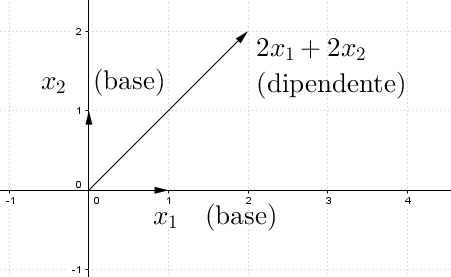
\includegraphics[width=0.4\linewidth]{img/vettori_dipendenti}\\
Possiamo notare che in questo caso, ogni punto nel piano può essere rappresentato come combinazione lineare dei due vettori base.\\

\noindent\textbf{Esercizio:} verificare che
\[
	2 + 3i
\]
sia linearmente indipendente (ovvero che genera tutto lo spazio):
\begin{gather*}
	x(2+3i) + yi = 0 \qquad \text{se si, sono linearmente indipendenti}\\
	2x + 3xi + yi = 0 \to
	\begin{cases*}
		x=0 \\
		y=0
	\end{cases*}
	\to
	\text{sono linearmente indipendenti e generano tutto lo spazio}
\end{gather*}
La base in questo caso non è un numero $\in \ins{R}$, ma $\in \ins{C}$.

\newpage
\noindent
Sia $V$ uno spazio vettoriale di base $V_1, ..., V_k$. Allora ogni insieme di elementi $W_1,...,W-n$ con $n>k$ è linearmente dipendente:\\\\
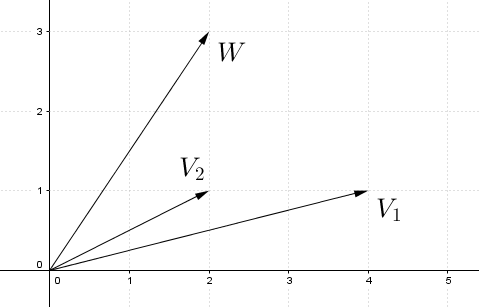
\includegraphics[width=0.4\linewidth]{img/vettori_dipendenti_1}\\
dove
\begin{gather*}
	W = c_1 \cdot V_1 + c_2 \cdot V_2 \\
	W = - c_1 \cdot V_1 - c_2 \cdot V_2 = 0
\end{gather*}
In particolare le due basi hanno lo stesso numero di elementi. Questo numero è la dimensione dello spazio vettoriale (2 in questo caso).
\[
	W_i = \underbracket{a_{1i}}_{\mathclap{\text{scalare}}}\cdot V_1 + ... + a\overbracket{_{ki}}^{\mathclap{\text{2 indici}}} \cdot \underbracket{V_k}_{\mathclap{\text{base}}} \qquad \text{con } 1\leq i \leq n
\]
Dati i due indici, possiamo ricavare una matrice dei coefficienti:
\[
	\begin{tikzpicture}[decoration=brace]
		\matrix (m) [matrix of math nodes,left delimiter=[,right delimiter={]}] {
			a_{11} & a_{12} & \dots & a_{1n} \\
			a_{21} & a_{22} & \dots & a_{2n} \\
			\text{$\vdots$} & \text{$\vdots$} &  & \text{$\vdots$} \\
			a_{k1} & a_{k2} & \dots & a_{kn} \\
		};
		
		\draw[decorate,transform canvas={xshift=-1.5em},thick] (m-4-1.south west) -- node[left=2pt] {$k$ righe} (m-1-1.north west);
		
		\draw[decorate,transform canvas={yshift=0.5em},thick] (m-1-1.north west) -- node[above=2pt] {$W_1$} (m-1-1.north east);
		
		\draw[decorate,transform canvas={yshift=0.5em},thick] (m-1-4.north west) -- node[above=2pt] {$W_n$} (m-1-4.north east);	
		
		\draw[decorate,transform canvas={yshift=-7em},thick] (m-1-4.north east) -- node[below=2pt] {$n$ colonne} (m-1-1.north west);	
		
	\end{tikzpicture}
\]
\\\\
e data la matrice dei coefficienti possiamo ricavare:
\begin{gather*}
	\begin{bmatrix}
		V_1 & \dots & V_k
	\end{bmatrix}
	\cdot
	\begin{bmatrix}
			a_{11} & a_{12} & \dots & a_{1n} \\
			a_{21} & a_{22} & \dots & a_{2n} \\
			\vdots & \vdots &  & \vdots \\
			a_{k1} & a_{k2} & \dots & a_{kn}
	\end{bmatrix}
	=
	\begin{bmatrix}
		W_1 & \dots & W_n
	\end{bmatrix}
\end{gather*}
a cui segue
\begin{gather*}
	0 =
	\begin{bmatrix}
		W_1 & \dots & W_n
	\end{bmatrix}
	\cdot
	\begin{bmatrix}
		x_1 \\ \vdots \\ x_n
	\end{bmatrix}
	=
	\begin{bmatrix}
		V_1 & \dots & V_k
	\end{bmatrix}
	\cdot
	\begin{bmatrix}
		a_{11} & a_{12} & \dots & a_{1n} \\
		a_{21} & a_{22} & \dots & a_{2n} \\
		\vdots & \vdots &  & \vdots \\
		a_{k1} & a_{k2} & \dots & a_{kn}
	\end{bmatrix}
	\cdot
	\begin{bmatrix}
		x_1 \\ \vdots \\ x_n
	\end{bmatrix}
	=
	\begin{bmatrix}
		V_1 & \dots & V_k
	\end{bmatrix}
	\cdot
	\begin{bmatrix}
		0 \\ \vdots \\ 0
	\end{bmatrix}
	= 0
\end{gather*}
La cui rappresentazione significa
\[
	x_1 \cdot W_1 + ... + x_n \cdot W_n = 0
\]

\newpage
\noindent
\textbf{Le 2 regole principali sono:}\\[2mm]
(1) Ogni insieme di vettori linearmente indipendenti può essere esteso ad una base\\[1mm]
(2) Qualsiasi insieme di vettori che genera tutto lo spazio può essere ridotto ad una base
\begin{gather*}
	\text{Se } x_1, \dots , x_n \text{ sono vettori linearmente indipendenti, cosa manca per essere una base?}\\
	\text{Se i vettori generano tutto lo spazio, sono basi}\\\\
	\text{altrimenti } W \text{ (sottospazio generato da $x_1, \dots , x_n$, insieme delle combinazioni lineari)}\\
	W = \{ c_1 \cdot x_1 + \dots + c_n\cdot x_n : c_1,...,c_n \text{ sono scalari} \}\\
	V \supsetneq W \\
	x_1, \dots , x_n, \underbracket{c_1x_1, c_nx_n}_{\mathclap{x_{n+1}}} \qquad\text{aggiungo un elemento}\\
	x_{n+1} - c_1x_1 - \dots - c_nx_n = 0 \to \text{dipendenza lineare}\\
	x_1, \dots , x_n, x_{n+1} \in V \setminus W \\\\
	\text{In pratica}\\
	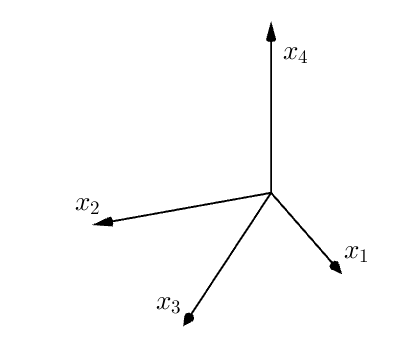
\includegraphics[width=0.3\linewidth]{img/basi}\\
	\text{dati i vettori $x_1, x_2$, aggiungo il vettore $x_3$, complanare a $x_1,x_2$.}\\
	\text{Ma dato che } x_3 - c_1x_1 - x_2 = 0 \text{ definisce un vettore dipendente, devo sostituire a $x_3$ un vettore che non sia}\\ 
	\text{dipendente da $x_1$ e $x_2$.}\\
	\text{Sostituisco a $x_3$ il vettore $x_4$, che non complanare ai primi due.}\\
	\text{Fatto ciò osservo che i 3 nuovi vettori sono linearmente indipendenti, e generano tutto lo spazio.}\\ 
	\text{Se generano tutto lo spazio, sono base.}
\end{gather*}

\newpage
\subsection{Tutorato}
\subsubsection{Esercizio 1}
Dimostrare che l'insieme dei polinomi a coefficienti razionali di grado al più 5 è uno spazio vettoriale con l'operazione $+$.
\begin{gather*}
	\begin{rcases*}
		a_0x^5 + ... + a_5 \\
		b_0x^5 + ... + b_5 \\
		c_0x^5 + ... + c_5 \\
	\end{rcases*}
	a,b,c \in \ins{Q} \text{ (numeri razionali)}
\end{gather*}
In pratica sommando polinomi di grado massimo 5, ottengo comunque polinomi di grado al più 5, quindi forma uno spazio vettoriale.

\subsubsection{Esercizio 2}
Un campo numerico è diverso da uno spazio vettoriale:\\
campo numerico: $(\ins{R}, + , \cdot)$ è un campo numerico perché ogni numero $\neq$ 0 è invertibile\\
spazio vettoriale: $(\ins{R}, +)$ è spazio vettoriale su $(\ins{R}, + , \cdot)$

\subsubsection{Esercizio 3}
I polinomi di grado $\leq$ 1 su \ins{Z}, formano uno spazio vettoriale su \ins{Z}?
\begin{gather*}
	\text{Poiché \ins{Z} non ha la proprietà dell'inverso (solo 1 è invertibile)}\\
	\text{non è un campo numerico. Se non è campo numerico, non è nemmeno spazio vettoriale}
\end{gather*}

\subsubsection{Esercizio 4}
Dimostrare che l'insieme delle soluzioni di
\[
	2x-3y+z = 0
\]
è sottospazio vettoriale di $\ins{R}^3$\\[2mm]
\textbf{Soluzione}:
\begin{gather*}
	U = \{ \text{insieme delle soluzioni di } 2x-3y+z = 0 \}
	\text{es.}\\
	(0,0,0) \in U\\
	(1,1,1) \in U\\
	(1,0,-2) \in U\\
	\dots
\end{gather*}
Ora dimostriamo che $U$  è sottospazio vettoriale di $\ins{R}^3$:
\begin{enumerate}
	\item verifichiamo che $U$ contenga lo zero:
		\begin{gather*}
		0 \in U \qquad \checkmark
		\end{gather*}
	\item verifichiamo che $x + y \in U $
		\begin{gather*}
			x,y \in U\\
			x=(a,b,c) \qquad 2a - 3b + c = 0 \\
			y=(m,n,p) \qquad 2m - 3n + p = 0 \\[1mm]
			\text{Ora dimostro che $(a,b,c) + (m,n,p) = (a+m,b+n,c+p) \in U$}\\[1mm]
			\underbracket{2a - 3b + c}_{0} + \underbracket{2m - 3n + p}_{0}= 0\\
			2(a+m)- 3(b+n) + (c+p) = 0\\[1mm]
			\text{La somma di due vettori rimane ancora nello stesso spazio vettoriale, quindi $ (a+m,b+n,c+p) \in U \qquad \checkmark$}
		\end{gather*}
	\pagebreak
	\item $k \in \ins{R} \;,\; x=(a,b,c) \in U$. Dimostrare che $kx = (ka,kb,kc) \in U$
	\begin{gather*}
		k(2a-3b+c)=k\cdot 0\\
		\begin{split}
			2\underbracket{ka}-3\underbracket{kb}+\underbracket{kc} &= k\cdot 0\\
			&= 0
		\end{split}\\
		\text{$(ka,kb,kc)$ sono le coordinate del vettore $k$, e ho dimostrato trovando le sue coordinate}\\
		\text{che è nello stesso spazio vettoriale delle soluzioni.}  \qquad \checkmark
	\end{gather*}
\end{enumerate}

\subsubsection{Esercizio 5}
Dimostrare che l'insieme delle soluzioni di
\[
	2x-3y+z = 1
\]
è sottospazio vettoriale di $\ins{R}^3$\\[2mm]
\textbf{Soluzione}:
\begin{gather*}
	U =  \{ \text{insieme delle soluzioni di } 2x-3y+z = 1 \}\\
	\text{E' sottospazio vettoriale di }\ins{R}^3 \text{? }
	\text{No, perché } 0 \notin U \qquad \crossmark
\end{gather*}

\subsubsection{Vettori linearmente indipendenti}
Due vettori $v,w$ sono linearmente \underline{dipendenti} se per ogni combinazione lineare
\[
	\lambda v + \mu w = 0 \qquad \text{con } \lambda,\mu \in \ins{R}
\]
Due vettori $v,w$ sono linearmente \underline{indipendenti} se per ogni combinazione lineare
\begin{gather*}
	\exists \lambda,\mu \in \ins{R} \text{ per cui }\lambda v + \mu w = 0	\\
	\land \; (\lambda \neq 0 \; \lor \; \mu \neq 0)
\end{gather*}

\subsubsection{Esercizio 5}
Dimostrare $(1,1)$ e $(2,2)$ sono linearmente dipendenti.\\[2mm]
\textbf{Soluzione}:
\begin{gather*}
	c_1 
	\begin{bmatrix}
		 1 \\ 1
	\end{bmatrix}
	+
	c_2
	\begin{bmatrix}
		2 \\ 2
	\end{bmatrix}
	= 0\\\\
	\begin{rcases*}
		c_1 = -2\\
		c_2 = 1
	\end{rcases*}
	\to
	-2
	\begin{bmatrix}
	1 \\ 1
	\end{bmatrix}
	+
	1
	\begin{bmatrix}
	2 \\ 2
	\end{bmatrix}
	= 0 \qquad \checkmark
\end{gather*}
Dato che $c_1,c_2 \neq 0$, i vettori sono linearmente dipendenti 

\subsubsection{Esercizio 6}
Dimostrare $(1,1)$ e $(0,1)$ sono linearmente indipendenti.\\[2mm]
\textbf{Soluzione}:
\begin{gather*}
	c_1 
	\begin{bmatrix}
		1 \\ 1
	\end{bmatrix}
	+
	c_2
	\begin{bmatrix}
		0 \\ 1
	\end{bmatrix}
	= 0\\\\
	\begin{rcases*}
		c_1 = 0\\
		c_2 = 0
	\end{rcases*}
	\to
	0
	\begin{bmatrix}
		1 \\ 1
	\end{bmatrix}
	+
	0
	\begin{bmatrix}
		0 \\ 1
	\end{bmatrix}
	= 0 \qquad \checkmark
\end{gather*}
Dato che $c_1,c_2 = 0$, i vettori sono linearmente indipendenti 

\subsubsection{Esercizio 7}
I vettori $(1,1,2)$, $(1,-1,1)$ e $(2,0,3)$ sono linearmente dipendenti?\\[2mm]
\textbf{Soluzione}:
\begin{gather*}
c_1 
\begin{bmatrix}
	1 \\ 1 \\ 2
\end{bmatrix}
+
c_2
\begin{bmatrix}
	1 \\ -1 \\ 1
\end{bmatrix}
+
c_3
\begin{bmatrix}
	2 \\ 0 \\ 3
\end{bmatrix}
= 0
\end{gather*}
E almeno $c_1,c_2$ o $c_3$ devono essere $\neq 0$
\begin{gather*}
\begin{rcases*}
c_1 = 1\\
c_2 = 1 \\
c_3 = -1
\end{rcases*}
\to
1
\begin{bmatrix}
1 \\ 1 \\ 2
\end{bmatrix}
+
1
\begin{bmatrix}
1 \\ -1 \\ 1
\end{bmatrix}
-1
\begin{bmatrix}
2 \\ 0 \\ 3
\end{bmatrix}
= 0 \qquad \checkmark
\end{gather*}
Dato che $c_1,c_2$ o $c_3$ sono diversi da zero, i vettori sono linearmente dipendenti 

\newpage
\section{Applicazioni lineari}
Siano $V$, $W$ due sottospazi vettoriali su \ins{K}.\\
Una funzione $f: V \longmapsto W$ è un'applicazione lineare che trasforma i vettori $v$ in $w$ se:
\begin{enumerate}
	\item $f(x+y) = f(x) + f(y)$
	\item $f(x) = c\cdot f(x)$ dove $c$ è uno scalare:
			\[
				c_1\cdot x_1 + c_2\cdot x_2 \xrightarrow{f} c_1\cdot f(x_1) + c_2\cdot f(x_2)
			\]
\end{enumerate}

\subsection{Esempi di applicazioni lineari:}
\subsubsection{Esempio 1}
\begin{itemize}
	\item 	Matrice identità: $I(x) = x$
			\[
				V \xrightarrow{I} V 	
			\]
	\item Funzioni composte:
			\begin{gather*}
				f: V \longmapsto W \qquad g: W \longmapsto H\\
				f\circ g: V \longmapsto H \\
				\begin{split}
					g \circ f(x+y) &= g(f(x+y))\\
					&= g(f(x)+f(y))\\
					&= g(f(x)) + g(f(y))\\
					&= (g\circ f)x + (g \circ f)y
				\end{split}
			\end{gather*}
\end{itemize}
\subsubsection{Esempio 2: vettori}
\begin{gather*}
	\text{Dati due vettori:} \qquad \vec{x} = (3,2,-2)\qquad \vec{y}=(y_1,y_2,y_3)\\
	\text{e data la funzione: } \quad  f: \ins{R}^3 \longmapsto \ins{R}\\[2mm]
	\begin{split}
		f(\vec{y}) &= \vec{y}\cdot \vec{x}\\
		&= 3y_1 + 2y_2 - 2y_3
	\end{split}\\[2mm]
	\begin{split}
		2) \qquad f \bigr(c(y_1,y_2,y_3) \bigr) &= f(cy_1,cy_2,cy_3) \\
		&= 3cy_1 + 2cy_2 - 2cy_3 \\
		&= c\cdot (3y_1 + 2y_2 - 2y_3) \\
		&= c \cdot f(\vec{y}) \checkmark
	\end{split}\\[2mm]
	\begin{split}
		1) \qquad f(x_1+y_1, x_2+y_2,x_3+y_3) &= 3(x_1+y_1) + 2(x_2+y_2) - 2(x_3+y_3) \\
		&= 3x_1 + 3y_1 + 2x_2 + 2y_2 - 2x_3 - 2y_3 \\
		&= f(\vec{x}) + f(\vec{y}) \checkmark 
	\end{split}
\end{gather*}
\newpage
\noindent
\subsubsection{Esempio 3: R2 to R }
Applicazione lineare: $f: \ins{R}^2 \longmapsto \ins{R}$\\
Trovo le basi di $\ins{R}^2$:
\[
	(1,0) \qquad (0,1) \qquad \textit{basi canoniche}
\]
Per conoscere tutte le combinazioni lineari di $f$ mi basta conoscere le immagini (\textit{codominio}) delle basi:
\[
	f(1,0) = 3 \qquad f(0,1) = 4
\]
Ora posso conoscere tutte le combinazioni lineari di $f$:
\[
	\begin{split}
	 f[(6,-9)] &= f(6\cdot (1,0) - 9\cdot(0,1)) \\
	 &= 6\cdot f(1,0) - 9\cdot f(0,1) \\
	 &= 6\cdot 3 - 9 \cdot 4 \\
	 &= -18
	\end{split}
\]

\noindent
\subsubsection{Esempio 4: R2 to R3}
Siano $V$ e $W$ due spazi vettoriali di 2 e 3 dimensioni e siano $v_1, v_2 $ le basi di $V$, e $w_1,w_2,w_3$ le basi di $W$.
\[
	f: \ins{R}^2 \longmapsto \ins{R}^3
\]
Trovo le basi di $\ins{R}^3$ e $\ins{R}^2$:
\begin{gather*}
	\ins{R}^3: \qquad (1,0,0) \qquad (0,1,0) \qquad (0,0,1)\\
	\ins{R}^2: \qquad (1,0) \qquad (0,1)
\end{gather*}
Per conoscere tutte le combinazioni lineari di $f$ mi basta conoscere le immagini (\textit{codominio}) delle basi:
\begin{gather*}
	f(v_1) = 3w_1 + 5w_2 - 2w_3 \\
	f(v_2) = w_1 + w_3
\end{gather*}
Ora posso conoscere tutte le combinazioni lineari di $f$:
\[
	\begin{split}
		f(3v_1 + 2v_2) &= 3\cdot f(v_1) + 2\cdot f(v_2) \\
		&= 3\cdot(3w_1 + 5w_2 - 2w_3) + 2\cdot(w_1+w_3) \\
		&= 11w_1 + 15w_2 - 4w_3	
	\end{split}
\]

\newpage
\noindent
\subsection{Teorema}
Siano $V$ e $W$ due spazi vettoriali. La funzione
\[
	f: V \longmapsto W
\]
è un'applicazione lineare.
\\\\
Trovo le immagini di $f$:
\begin{gather*}
	\begin{split}
		cod(f) &= \{ w \in W : \exists v\in V \quad f(v)=w \} \\
		&= \{ f(v) : v \in V \}\qquad \textit{insieme degli output}
	\end{split}
\end{gather*}
Determino il kernel (\textit{nucleo}), ovvero tutti i vettori che vanno in zero:
\[
	ker(f) = \{ v \in V : f(v)= \underline{0} \}
\]
cioè l'insieme degli elementi del dominio $V$ che hanno immagine \underline{0} mediante $f$.
\subsubsection{Regole}
\begin{enumerate}
	\item \imm{f} è sottospazio di $W$
	\item \ker{f} è sottospazio di $V$ 
	\item \dim{V} = $\text{dim } ker(f) + \text{dim } Imm(f)$
\end{enumerate}

\noindent
\subsubsection{Esempio 1}
Una funzione $f: \ins{R}^3 \longmapsto \ins{R}$
\begin{gather*}
	f(y_1,y_2,y_3) = 3y_1 + 2y_2 - 2y_3 \\\\
	3 = \underbracket{\text{dim } ker(f)}_{\mathclap{\ins{R}^3 -\ins{R}^1 \to 3-1 = 2}} + \underbracket{\text{dim } Imm(f)}_{\mathclap{\ins{R}^1 = 1}}
\end{gather*}

\noindent
\subsubsection{Esempio 2}
Data una funzione $f: \ins{R}^2 \longmapsto \ins{R}^3$ dove
\begin{itemize}
	\item $v_1,v_2$ sono base di $\ins{R}^2$
	\item $w_1,w_2,w_3$ sono base di $\ins{R}^3$
\end{itemize}
La funzione è definita come $f: V \longmapsto W$ ed è un'applicazione lineare.
\begin{gather*}
	f(v_1) = 4w_1 + w_2 + w_3 \\
	f(v_2) = w_1 + 2w_3\\\\
	f(c_1v_1 + c_2v_2) = c_1 \cdot f(v_1) + c_2 \cdot f(v_2)
\end{gather*}
Costruisco la matrice associata:
\[
	\begin{bmatrix}
		4 & 1 \\
		1 & 0 \\
		1 & 2
	\end{bmatrix}
	\cdot
	\begin{bmatrix}
	c_1 \\ c_2
	\end{bmatrix}
	=
	\begin{bmatrix}
		4c_1 + c_2 \\
		c_1 \\
		c_1 + 2c_2
	\end{bmatrix}
\]
dove la prima riga indica la coordinata rispetto a $w_1$, la seconda e $w_2$ e la terza a $w_3$. I coefficienti vanno messi in colonna.\\[3mm]
\textit{Prova}:
\[
	\begin{split}
		f(c_1v_1 + c_2v_2) &= c_1(4w_1 + w_2 + w_3) + c_2(w_1 + 2w_3)\\
		&= c_1 \cdot f(v_1) + c_2 \cdot f(v_2)
	\end{split}
\]

\newpage
\noindent
\subsection{Costruzione matrice associata}
\[
	f(v_1) = \sum_{i=1}^{k}aw_{i1} = a_{11}w_ 1 + ... + a_{k1}w_k
\]
dove possiamo notare che vi sono due indici, che indicano quindi una matrice:
\[
	\begin{bmatrix}
		a_{11} & \dots & a_{1n} \\
		a_{21} & \dots & a_{2n} \\
		\vdots & & \\
		a_{k1} & \dots & a_{kn}
	\end{bmatrix}
\]
\subsubsection{Esempio}
Trovare l'applicazione lineare da $\ins{R}^4 \xrightarrow{f} \ins{R}^3$ che soddisfi
\[
	A = 
	\begin{bmatrix}
		3 & 4 & 2 & 1 \\
		4 & -6 & 0 & 0 \\
		1 & 2 & -2 & 2
	\end{bmatrix}
	\cdot
	\begin{bmatrix}
		x_1 \\ \vdots \\ x_4
	\end{bmatrix}
\]
Trovo le basi di $\ins{R}^4$:
\begin{itemize}
	\item $e_1 = (1,0,0,0)$
	\item $e_2 = (0,1,0,0)$
	\item $e_3 = (0,0,1,0)$
	\item $e_4 = (0,0,0,1)$
\end{itemize}
Trovo le basi di $ \begin{bmatrix} x_1 \\ ... \\ x_4 \end{bmatrix}$, ovvero $\ins{R}^3$:
\begin{itemize}
	\item $e_1' = (1,0,0)$
	\item $e_2' = (0,1,0)$
	\item $e_3' = (0,0,1)$
\end{itemize}

\begin{gather*}
	\begin{split}
		f(e_1) &= 
		\begin{bmatrix}
			3 & 4 & 2 & 1 \\
			4 & -6 & 0 & 0 \\
			1 & 2 & -2 & 2
		\end{bmatrix}
		\cdot
		\begin{bmatrix}
			1 \\ 0 \\ 0 \\ 0
		\end{bmatrix}
		=
		\begin{bmatrix}
			3 \\ 4 \\ 1
		\end{bmatrix}\\
		&= 3e_1' + 4e_2' + e_3'
	\end{split} \\\\
	\begin{split}
		f(e_2) &= 
		\begin{bmatrix}
			3 & 4 & 2 & 1 \\
			4 & -6 & 0 & 0 \\
			1 & 2 & -2 & 2
		\end{bmatrix}
		\cdot
		\begin{bmatrix}
			0 \\ 1 \\ 0 \\ 0
		\end{bmatrix}
		=
		\begin{bmatrix}
			4 \\ -6 \\ 2
		\end{bmatrix}\\
		&= 4e_1' - 6e_2' + 2e_3'
	\end{split} \\\\
	\dots
\end{gather*}

\newpage
\subsection{Applicazione lineare da matrice}
Sia $V$ spazio vettoriale di base $v_1, ... , v_n$ e sia $W$ spazio vettoriale di base $w_1, ... , w_m$. Sia $A$ una matrice di $m$ righe e $n$ colonne.
\[
	f: V \xrightarrow{f_A} W
\]
La rappresentazione: \textcolor{red}{\textbf{vedi pag. 54 SALPDF}}
\begin{gather*}
	A^1 \text{ indica la prima colonna} \\ 
	A_1 \text{ indica la prima riga}
\end{gather*}
Generazione matrice:
\begin{gather*}
	\begin{split}
		A\cdot
		\begin{bmatrix}
		c_1 \\ \vdots \\ c_n
		\end{bmatrix}
		&= 
		\begin{bmatrix}
			A^1,A^2, ..., A^n
		\end{bmatrix}
		\cdot
		\begin{bmatrix}
			c_1 \\ \vdots \\ c_n
		\end{bmatrix} \\\\
		&= 
		\begin{bmatrix}
			A_1, A_2, ... , A_n
		\end{bmatrix}
		\cdot
		\begin{bmatrix}
			c_1 \\ \vdots \\ c_n
		\end{bmatrix} \\\\
		&=
		\begin{bmatrix}
			A_1 \cdot \vec{c} \\
			A_2 \cdot \vec{c} \\
			\vdots \\
			A_n \cdot \vec{c}		
		\end{bmatrix} \\\\
		&= 
		\begin{bmatrix}
			\sum_{i=1}^{n} a_{1i} \cdot c_i \\
			\sum_{i=1}^{n} a_{2i} \cdot c_i \\
			\vdots \\
			\sum_{i=1}^{n} a_{mi} \cdot c_i
		\end{bmatrix}
	\end{split}
\end{gather*}
La matrice $A$ determina:
\begin{itemize}
	\item il sottospazio generato dalle righe: $A_1,...,A_m \subseteq V$
	\item il sottospazio generato dalle colonne: $A^1,...,A^n \subseteq W$
	\item il sottospazio generato dalle colonne e dalle righe è lo stesso:
		\begin{gather*}
			\text{dim}(Imm \; f_A) = \langle A^1, ... , A^n \rangle \\
			n = \text{numero di colonne} \\
			n = \text{dim}(ker \; f_A) + \text{dim(\textit{spazio colonne})} \\\\
			\langle A^1, ... , A^n \rangle \subseteq V \\
			\langle A^1, ... , A^n \rangle \text{ è ortogonale al nucleo }ker(f_A) \\
			n = \text{dim}(ker \; f_A) + \text{dim } \langle A^1, ... , A^n \rangle 
		\end{gather*}
\end{itemize}

\newpage
\tright{19-11-2015}
Applicazione lineare:
\[
	f: V \longmapsto W
\]
dove 
\begin{gather*}
	v_1,...,v_n \in V \\
	w_1,...,w_m \in W \\\\
	\dim{V} = n \\
	\dim{W} = m
\end{gather*}
La matrice associata avrà dimensione $m \times n$
\[
	f(v_i) = \sum_{k=1}^{m}a_{ki}w_k \text{ nella matrice } A = 
	\begin{bmatrix}
		a_{1i} \\ a_{2i} \\ \vdots \\ a_{mi}
	\end{bmatrix}
\]

\subsection{Isomorfismi}
Quando un'applicazione lineare è un isomorfismo?\\
$f: V \longmapsto W$ è un isomorfismo lineare sse $f$ è un'applicazione lineare biettiva:\\[2mm]
$f^{-1}: W \longmapsto V$  è un isomorfismo lineare tale che
\begin{gather*}
	f \circ f^{-1} = I_V = f^{-1} \circ f \\
	I_V: V \longmapsto V \\
	I_V(\underline{x}) = \underline{x} 
\end{gather*}
\noindent
Due spazi vettoriali che hanno la stessa dimensione sono isomorfi se sono sullo stesso campo numerico:\\
es.
\begin{table}[h]
	\begin{tabular}{cccc}
		   & $\ins{R}^4$       	& $P^3[x]$ 		& matrici $2\times 2$ \\[5mm]
		   
		$e_1$  & $(0,0,0,1)$	& $1$   		& $\begin{bmatrix} 1 & 0 \\ 0 & 0 \end{bmatrix}$      
		  \\[5mm]
		$e_2$  & $(0,0,1,0)$    & $x$   		& $\begin{bmatrix} 0 & 1 \\ 0 & 0 \end{bmatrix}$           \\[5mm]
		$e_3$  & $(0,1,0,0)$    & $x^2$   		& $\begin{bmatrix} 0 & 0 \\ 1 & 0 \end{bmatrix}$           \\[5mm]
		$e_4$  & $(1,0,0,0)$    & $x^3$    		& $\begin{bmatrix} 0 & 0 \\ 0 & 1 \end{bmatrix}$          
	\end{tabular}
\end{table}
\begin{gather*}
	e_1 \longmapsto 1 \\
	e_2 \longmapsto x \\
	e_3 \longmapsto x^2 \\
	e_4 \longmapsto x^3
\end{gather*}
Esempio numerico : 
\[
	v=(2,2,1,0) \longmapsto 2 + 2x + x^2 \text{ è bigettiva, quindi è un isomorfismo}
\]

\newpage
\subsubsection{Teorema} due spazi vettoriali con la stessa dimensione sono isomorfi.\\
Il nucleo di un'applicazione lineare isomorfa è: \[ \ker{f} = \{ 0 \} \]
Un'applicazione lineare è iniettiva sse $\ker{f} = \{ 0 \}$
Una matrice quadrata è invertibile quando $f_A$ è isomorfa (ovvero quando è associata ad un'applicazione lineare isomorfa).\\
Es.
\begin{gather*}
	f: V \longmapsto W \qquad\qquad A = m \times n \\
	g: W \longmapsto H \qquad\qquad B = r \times m \\
	g \circ f: V \longmapsto H \qquad\quad BA = r \times n
\end{gather*}


\subsubsection{Cambio di base} esempio in $\ins{R}^2$
\begin{gather*}
	e_1 = (0,1) \qquad w_1(1,2) \\
	e_2 = (1,0) \qquad w_2 = (3,1)
\end{gather*}
Voglio cambiare la base canonica $e_1,e_2$ con la base $w_1,w_2$.\\
Una volta controllato che $w_1,w_2$ siano linearmente indipendenti:
\begin{gather*}
	e_1 = c_1w_1 + c_2w_2 \\
	e_2 = d_1w_1 + d_2w_2 \\\\
	\begin{bmatrix}
		c_1 & d_1 \\
		c_2 & d_2
	\end{bmatrix}
	\begin{bmatrix}
		1 \\ 0
	\end{bmatrix}
	=
	\begin{bmatrix}
		c_1 \\ c_2
	\end{bmatrix} \\\\
	(1,0) = c_1(1,2) + c_2(3,1) \\\\
	\begin{cases*}
		1 = c_1 + 3c_2 \\
		0 = 2c_1 + c_2
	\end{cases*}
	\begin{cases*}
		c_1 = -\frac{1}{5} \\
		c_2 = \frac{2}{5}
	\end{cases*} \\\\
	\begin{split}
		(1,0) &= -\frac{1}{5}(1,2) + \dfrac{2}{5}(3,1) \\
		&= (-\frac{1}{5} + \frac{6}{5}, -\frac{2}{5} + \frac{2}{5}) \\
		&= (1,0) \checkmark
	\end{split} \\\\
	\text{Ripeto lo stesso procedimento con } d_1, d_2 \\\\
	\begin{bmatrix}
		-\frac{1}{5} & d_1 \\
		\frac{2}{5} & d_2
	\end{bmatrix}
	\begin{bmatrix}
		1 \\ 0
	\end{bmatrix}
	=
	\begin{bmatrix}
		? \\ ?
	\end{bmatrix}
\end{gather*}

\newpage
\tright{19-11-2015}
Ogni matrice elementare in quanto invertibile determina un isomorfismo.\\\\
Data la matrice $A = m \times n$:
\[
	\begin{bmatrix}
		&&& \\ &A& \\ &&&
	\end{bmatrix}
	\begin{bmatrix}
		x_1 \\ \vdots \\ x_m
	\end{bmatrix}
	=
	\begin{bmatrix}
		0 \\ \vdots \\ 0_m
	\end{bmatrix} \qquad
	\ins{R}^n \xrightarrow{f_A} \ins{R}^m
\]
le soluzioni del sistema lineare omogeneo corrispondono al nucleo $\ker{f_A}$, che è sottospazio di $\ins{R}^n$.\\\\
Se $m=n$ ?? 
\begin{gather*}
	\ins{R}^n \xrightarrow{f_A} \ins{R}^n \xrightarrow{f_E} \ins{R}^m \\
	EA \qquad \ker{f_A \circ f_E} = \ker{f_A}
\end{gather*}
infatti moltiplicando per una matrice elementare non modifico lo spazio delle soluzioni, semplifico solamente la matrice.\\\\
altrimenti se $n>m$
\begin{gather*}
	n = \dim{\ker{f_A}} + \dim{\imm{f_A}}
\end{gather*}
\\\\
\textbf{Esempio}
\begin{gather*}
	\ins{R}^n \xrightarrow{f_A} \ins{R}^n \\\\
	\overset{m\times n}{	
		\begin{bmatrix}
			&&& \\ &A& \\ &&&
		\end{bmatrix}
	}
	\begin{bmatrix}
		x_1 \\ \vdots \\ x_m
	\end{bmatrix}
	=
	\begin{bmatrix}
		b_1 \\ \vdots \\ b_m
	\end{bmatrix}
	\qquad b \in \imm{f_A}\\\\
	EA 
	\begin{align*}
		&A\underline{x} = \underline{b} \\
		&EA\underline{x} = E\underline{b} \\
		& \ins{R}^n \xrightarrow{f_A} \ins{R}^n \xrightarrow{f_E} \ins{R}^m
	\end{align*}
\end{gather*}
il sistema ammette soluzioni: $(f_E \circ f_A)\underline{x} = E\underline{b}$\\\\

\newpage
\noindent
Esempio:
\[
	\begin{bmatrix}
		1 & 2 & 3 \\ 4 & 5 & 6 \\ 7 & 8 & 9
	\end{bmatrix}
	\begin{bmatrix}
		x_1 \\ x_2 \\ x_3
	\end{bmatrix}
	=
	\begin{bmatrix}
		0 \\ 0 \\ 0
	\end{bmatrix}
\]
risolvere questo sistema significa:
\begin{gather*}
	A_1 \cdot \underline{x} = 0 \\
	A_2 \cdot \underline{x} = 0 \qquad\qquad f_A: \underbracket{\ins{R}^3}_{\mathclap{\text{spazio righe}}} \longmapsto \overbracket{\ins{R}^3}^{\mathclap{\text{spazio colonne}}} \\
	A_3 \cdot \underline{x} = 0
\end{gather*}
ovvero trovare un vettore $x$ perpendicolare ad ogni vettore riga $A^1,A^2,A^3$, che a sua volta significa essere ortogonale al sottospazio generato dai vettori riga $A^1,A^2,A^3$. Questo implica che il vettore $x$ deve stare nel nucleo dell'applicazione lineare. Ma ogni vettore nel nucleo è perpendicolare ai vettori riga. Il nucleo $\ker{f_A}$ è quindi ortogonale al sottospazio generato dalle righe.

\subsubsection{Teorema}
sia $V$ uno spazio vettoriale, sia $u \subseteq V$ un sottospazio di $V$. Allora il sottospazio di $V$ ortogonale a $u$ è:
\[
	u^{\perp} = \{ x \in V : (\forall y \in u) x\cdot y = 0 \}
\]
verifica $\dim{V} = \dim{u} + \dim{u^{\perp}}$.\\\\

\noindent
Tornando all'esempio di prima:\\
lo spazio generato dalle righe è lo spazio $(\ker{f_A})^{\perp}$
\[
	\begin{split}
		\dim{V} &= \dim{\ker{f_A}} + \dim{\text{spazio delle righe}} \\	
		3 &= \dim{\ins{R}^3} \\
		&= \dim{\ker{f_A}} + \dim{\text{spazio delle righe}} \\
		&= \dim{\ker{f_A}} + \dim{\imm{f_A}} \\
		&= \dim{\ker{f_A}} + \dim{\text{spazio delle colonne}} 
	\end{split}
\]

\newpage
\subsection{Il determinante}
Data una matrice quadrata $A = m\times n$, il $\det{A}$ appartiene campo numerico.
Proprietà:
\begin{enumerate}
	\item il determinante della matrice identica è 1:
			\[
				\det{I} = 1
			\]
	\item se due colonne contigue sono uguali:
			\[
				\det{A} = 0
			\]
	\item il determinate è lineare su ciascuna colonna:
			\begin{gather*}
				\det{A^1,...,A^n} \\
				\det{A^1,...,B+C,...,A^n} = \det{A^1,...,B,...,A^n} + \det{A^1,...,C,...,A^n} \\\\
				\det{A^1,...,c\cdot A^i,...,A^n} = c \cdot \det{A^1,...,A^n} \\\\
				\det{
					\begin{bmatrix}
						2 & 5 \\ 1 & 1
					\end{bmatrix}
				} =
				\det{
					\begin{bmatrix}
						2 & 5 \\ 1 & 0
					\end{bmatrix}
				}
				+
				\det{
					\begin{bmatrix}
						2 & 1 \\ 0 & 1
					\end{bmatrix}
				}
			\end{gather*}
	\item il determinante di una matrice diagonale è la il prodotto della diagonale stessa
	\item se due colonne contigue vengono scambiate, il determinate cambia segno:
			\[
				\det{A^1,A^2} = -\det{A^2,A^1}
			\]
	\item se le colonne $A^i$ e $A^j$ con $i\neq j$ sono uguali, $\det{A} = 0$
	\item se si sommano ad una colonna un multiplo scalare di un'altra colonna, il determinante non cambia
\end{enumerate}

\subsubsection{Calcolo del determinante}
Calcolare il determinante della matrice
\[
	A =
	\begin{bmatrix}
		1 & 2 \\ 3 & 4
	\end{bmatrix}
\]
il determinante della matrice $A$ si indica anche come $\det{A} = |A|$.
\begin{gather*}
	\begin{split}
		\det{A} &=
		\begin{vmatrix}
			 \begin{pmatrix}
				 1 \\ 0
			 \end{pmatrix}
			 +
			 \begin{pmatrix}
				 0 \\ 3
			 \end{pmatrix} 
			 & 
			 \begin{matrix}
			  2\; \\ 4\;
			 \end{matrix}
		\end{vmatrix} 
		\\[2mm]
		& = 
		 \begin{vmatrix}
			1 & 2 \\
			0 & 4
		\end{vmatrix}
		+ \begin{vmatrix}
			0 & 2 \\ 3 & 4 \;
		\end{vmatrix} 
		\\[2mm]
		&=
		\begin{vmatrix}
			\begin{matrix}
				1 \\ 0
			\end{matrix}
			&
			\begin{pmatrix}
				2 \\ 0
			\end{pmatrix}
			+
			\begin{pmatrix}
				0 \\ 4
			\end{pmatrix} 
		\end{vmatrix} 
		+
		\begin{vmatrix}
			\begin{matrix}
				0 \\ 3
			\end{matrix}
			&
			\begin{pmatrix}
				2 \\ 0
			\end{pmatrix}
			+
			\begin{pmatrix}
				0 \\ 4
			\end{pmatrix} 
		\end{vmatrix} 
		\\[2mm]
		&=
		\cancel{
			\begin{vmatrix}
				1 & 2 \\ 0 & 0
			\end{vmatrix}
		}
		+
		\begin{vmatrix}
			1 & 0 \\ 0 & 4
		\end{vmatrix}
		+
		\begin{vmatrix}
			0 & 2 \\ 3 & 0
		\end{vmatrix}
		+
		\cancel{
			\begin{vmatrix}
				0 & 0 \\ 0 & 4
			\end{vmatrix}
		}
		\\[2mm]
		&=
		\begin{vmatrix}
			1 & 0 \\ 0 & 4
		\end{vmatrix}
		+
		\begin{vmatrix}
			0 & 2 \\  3 & 0
		\end{vmatrix}
		\\[2mm]
		&= 1\cdot 4 - 0\cdot 0 + (0\cdot 0 - 2\cdot 3) \\[2mm]
		&= 4 - 6 \\[2mm]
		&= -2
	\end{split}
\end{gather*}
\newpage
\subsubsection{Regola di Cramer}
Con la regola di Cramer possiamo risolvere il sistema lineare $A\underline{x}=\underline{b}$ utilizzando i determinanti.\\\\
Sia $A$ una matrice $n\x n$ con determinante diverso da 0.\\Se $b$ è un vettore colonna e $c_1,...,c_n$ sono scalari tali che 
\[
	A\underline{c} = c_1A^1 + c_2A^2 + ... + c_nA^n
\]
allora abbiamo
\[
	c_i = \dfrac{\det{A^1,...,A^{i-1},b,A^{i+1},...,A^n}}{\det{A}}
\]

\subsubsection{Esercizio}
\[
	A = 
	\begin{bmatrix}
		1 & 2 \\ 3 & 4
	\end{bmatrix}
	\begin{bmatrix}
		c_1 \\ c_2
	\end{bmatrix}
	=
	\begin{bmatrix}
		2 \\ 3
	\end{bmatrix}
\]
Dobbiamo trovare $c_1$ e $c_2$:
\begin{gather*}
	c_1 = \dfrac{\begin{vmatrix} 2 & 2\\3 & 4\end{vmatrix}}{\det{A}} = -1\\[2mm]
	c_2 = \dfrac{\begin{vmatrix} 1 & 3\\2 & 3\end{vmatrix}}{\det{A}} = \frac{3}{2}
\end{gather*}
Regola del determinante
\begin{gather*}
	\begin{split}
	 \det{A} &= (-1)^{i+1}\cdot a_{i1}\cdot |A_{i1}|+(-1)^{i+2}\cdot a_{i2}\cdot |A_{i2}| + ... + (-1)^{i+n}\cdot a_{in}\cdot |A_{in}|\\
	 &= (-1)^{i+1}\cdot a_{1i}\cdot |A_{1i}|+(-1)^{i+2}\cdot a_{2i}\cdot |A_{2i}| + ... + (-1)^{i+n}\cdot a_{ni}\cdot |A_{ni}|
	\end{split}
\end{gather*}
Esempio
\begin{gather*}
		\left|
			\begin{array}{ccc}
				\tikzmarkin[ver=style green]{col 1}\textbf{0} & \tikzmarkin[hor=style green]{myrow2}1 & 1\tikzmarkend{myrow2}\\
				2 & 1 & 4 \\
				3\tikzmarkend{col 1}  &  2  &  1 \\
			\end{array}
		\right|
		\qquad\text{quella non evidenzioata è la matrice } A_{11} \text{. Prendo l'elemento 11 e elimino la sua riga e colonna}\\\\
		\text{Calcolo del determinante rispetto alla riga 2:}\\
	\begin{split}
		\begin{vmatrix}
			\;0 & 1 & 1 \\ \textcolor{red}{2} & \textcolor{red}{1} & \textcolor{red}{4} \\ 3 & 2 & 1\;
		\end{vmatrix} 
		&= 
		(-1)^{i+1}\cdot \textcolor{red}{2}|A_{i1}| + (-1)^{i+2}\cdot \textcolor{red}{1}|A_{i2}| + (-1)^{i+3}\cdot \textcolor{red}{4}|A_{i3}|\\[2mm]
		i=2: \qquad &=
		(-1)^{2+1}\cdot 2\begin{vmatrix}1&1\\2&1\end{vmatrix} + (-1)^{2+2}\cdot 1\begin{vmatrix}0&1\\3&1\end{vmatrix} + (-1)^{2+3}\cdot 4\begin{vmatrix}0&1\\3&2\end{vmatrix} \\[2mm]
		&= -2\begin{vmatrix}1&1\\2&1\end{vmatrix} + \begin{vmatrix}0&1\\3&1\end{vmatrix} -4\begin{vmatrix}0&1\\3&2\end{vmatrix} \\[2mm]
		&= -2\cdot (-1) -3 + 12 = 12 - 1 = 11
	\end{split}
\end{gather*}
\newpage
\subsubsection{Esercizio}
Calcolare il determinante della matrice
\[
	\begin{bmatrix}
		1 & 2 & 2 & 2 \\ 3 & 1 & 1 & 2 \\ 4 & 0 & 5 & 1 \\ 0 & 1 & 1 & 0
	\end{bmatrix}
\]
Devo scegliere una riga dalla quale partire. Mi conviene prendere quella con più zeri possibile. In questo caso l'ultima riga. Per facilitare ancora di più sottraggo la 3 riga dalla seconda, e ottengo:
\[
	\begin{bmatrix}
		1 & 0 & 2 & 2 \\ 3 & 0 & 1 & 2 \\ 4 & -5 & 5 & 1 \\ 0 & 0 & 1 & 0
	\end{bmatrix}
\]
a questo punto scelgo come riga per calcolare il determinante la quarta:
\begin{gather*}
		\left|
			\begin{array}{cccc}
				1 & 0 & \tikzmarkin[ver=style green]{col 3}2 & 2 \\ 
				3 & 0 & 1 & 2 \\ 4 & -5 & 5\tikzmarkend{col 3} & 1 \\
				\tikzmarkin[hor=style green]{el}0 & 0 & \textbf{1} & 0\tikzmarkend{el}
			\end{array}
		\right|
		=
		\underset{pos}{-}1\cdot
		\left|
			\begin{array}{ccc}
				1 & 0 & 2 \\
				3 & 0 & 2 \\
				4 & -5 & 1
			\end{array}
		\right|
\end{gather*}
poi utilizzo la 1 riga, che ha più zeri delle altre:
\begin{gather*}
	\begin{split}
		-
		\left|
			\begin{array}{ccc}
				\textbf{1} & 0 & \textbf{2} \\
				3 & 0 & 2 \\
				4 & -5 & 1
			\end{array}
		\right|
		&=
		-
		\left(
			\textbf{1}
			\begin{vmatrix}
				0 & 2 \\
				-5 & 1
			\end{vmatrix}
			+
			\textbf{2}
			\begin{vmatrix}
				3 & 0 \\
				4 & -5
			\end{vmatrix}	
		\right) = 
		-(10 + 2\cdot(-15)) = -(10 - 30) = 20
	\end{split}
\end{gather*}
\underline{Il determinante della matrice è $20$.}\\\\
I segni "$-$" evidenziati con \textit{pos} sono quelli derivanti dalla posizione del numero. Sommo indice riga e colonna, se sono dispari il segno è negativo, positivo altrimenti.

\subsubsection{Determinante di un applicazione lineare}
Sia $f: V \longmapsto W$ un'applicazione lineare. Sia $v_1,...,v_n$ una base e sia $A$ la matrice $n \x n$ che rappresenta $f$ rispetto a $v_1,...,v_n$.

Se consideriamo un'altra base di $V$, $w_1,...,w_n$, allora consideriamo la matrice $B$ che rappresenta $f$ rispetto a questa nuova base. Sappiamo inoltre che esiste una matrice invertibile associata al cambiamento di base, che chiameremo matrice $C$. 
Cosi abbiamo:
\[
	B = C^{-1}AC
\]
e quindi 
\[
	|B| = |C^{-1}|\cdot |A| \cdot |C| = |A|
\]
Segue che \textbf{il determinante di una applicazione lineare $f$ è indipendente dalla scelta della base} (e quindi della matrice che rappresenta $f$).\\\\
Data una applicazione lineare $f$, possiamo scrivere quindi $\det{f}$, intendendo con questo il determinante di una qualsiasi matrice che rappresenta $f$.\\\\
\[
	\underset{\mathrlap{C}}{
		\underset{\mathclap{v_1,...,v_n}}{V} \quad \overset{I}{\longmapsto} \quad
	}   
	\underset{\mathclap{B}}{
		\underset{\mathclap{w_1,...,w_n}}{V}
		 \quad \overset{f}{\longmapsto} \quad \underset{\mathclap{w_1,...,w_n}}{V}
	}
	 \quad \overset{I}{\longmapsto} \quad  \underset{\mathclap{v_1,...,v_n}}{V}
\]

\subsubsection{Esercizio}
Data l'applicazione lineare identica $I: \underset{v_1,v_2}{\ins{R}^2} \longmapsto \underset{w_1,w_2}{\ins{R}^2}$.
\begin{gather*}
	v_1 = (1,1) \qquad w_1 = (1,-1)\\
	v_2 = (0,1) \qquad w_2 = (-1,-1)\\\\
	I(v_1) = v_1 = c_1w_1 + c_2w_2 = -w_2 \\
	I(v_2) = v_2 = d_1w_1 + d_2w_2 = d_1w_1 + d_2w_2 \\\\
	d_1\begin{bmatrix}1\\-1\end{bmatrix} + d_2\begin{bmatrix}-1\\-1\end{bmatrix} = \begin{bmatrix}0\\1\end{bmatrix} \\\\
	\begin{cases*}
		d_1 - d_2 = 0 \\
		-d_1 - d_2 = 1
	\end{cases*}
	\qquad\begin{cases*}
		d_1 = d_2 \\
		-d_2 - d_2 = 1
	\end{cases*}
	\qquad
	\begin{cases*}
		d_1 = d_2 \\
		d_2 = - \frac{1}{2}
	\end{cases*}
	\qquad
	\begin{cases*}
		d_1 = - \frac{1}{2} \\
		d_2 = - \frac{1}{2}
	\end{cases*} \\\\
	-\frac{1}{2} \begin{bmatrix}1\\-1\end{bmatrix} -\frac{1}{2}\begin{bmatrix}-1\\-1\end{bmatrix} =
	\begin{bmatrix}0\\1\end{bmatrix} \\\\
	\begin{bmatrix}0 & -\dfrac{1}{2} \\[3mm] -1 & -\dfrac{1}{2}\end{bmatrix} \textcolor{red}{???}
\end{gather*}

\subsubsection{Altre proprietà del determinante}
\begin{gather*}
	\det{A^T} = \det{A} \\
	\det{AB} = \det{A} \cdot \det{B}\\
	\det{A^{-1}} =\det{A}^{-1} = \frac{1}{\det{A}} 
\end{gather*}

\newpage
\subsection{Autovettori e autovalori}
Sia $V$ uno spazio vettoriale e sia $f: V \longmapsto V$ un'applicazione lineare. Un \textit{autovettore} è un elemento non nullo $v \in V$ per cui esiste uno scalare $\lambda$ tale che
\[
	f(v) = \lambda v \qquad \text{dilato o restringo il vettore }v
\]
Lo scalare $\lambda$ viene detto autovalore.\\\\
Se $A$ è una matrice che rappresenta un'applicazione lineare $f$ rispetto ad una base $v_1,...,v_n$, e l'autovettore ha coordinate $v = c_1v_1 + ... + c_nv_n$, allora
\[
	A
	\begin{bmatrix}
		c_1 \\ \vdots \\ v_n
	\end{bmatrix}
	= 
	\lambda
	\begin{bmatrix}
		c_1 \\ \vdots \\ c_n
	\end{bmatrix}
\]
l'autovalore $\lambda$ e l'autovettore $v$ sono detti autovalore e autovettore della matrice $A$.\\\\
Esempio. Se $V$ è uno spazio vettoriale sul campo \ins{R}, $v$ è un autovettore di autovalore sse
\begin{gather*}
	f(cv) = c\cdot \lambda v \qquad \textit{ovvero se trasforma rette in rette, dilatandole $(\lambda > 1)$ o contraendole $ (0 <\lambda < 1)$}
\end{gather*}

\noindent
\textbf{Condizioni equivalenti}\\
\begin{gather*}
		A\begin{bmatrix}c_1 \\ \vdots \\ c_n\end{bmatrix} = \lambda \begin{bmatrix}c_1 \\ \vdots \\ c_n\end{bmatrix} = \begin{bmatrix}\lambda c_1 \\ \vdots \\ \lambda c_n\end{bmatrix} \\[2mm]
	A\begin{bmatrix}c_1 \\ \vdots \\ c_n\end{bmatrix}	= \lambda
		\overset{\text{matrice identica}}{
			\begin{bmatrix}
				1  & \dots & 0 \\
				\vdots & 1 &  0 \\
				0 & 0 & 1
			\end{bmatrix}
		}
		\begin{bmatrix}c_1 \\ \vdots \\ c_n\end{bmatrix}\\[2mm]
	(A - \lambda I)\begin{bmatrix}c_1 \\ \vdots \\ c_n\end{bmatrix} = \begin{bmatrix}0 \\ \vdots \\ 0\end{bmatrix}
\end{gather*}
In una matrice può esistere un autovalore sse esiste $\lambda$ nel campo numerico tale che $\det{A - \lambda I} = 0$
\subsubsection{Esercizio}
Determinare gli autovalori di
\[
	A = 
	\begin{bmatrix}
		1 & 2 \\ 3 & 4
	\end{bmatrix}
\]
Inizio a risolvere:
\begin{gather*}
	\begin{split}
		|A - \lambda I| &= 
		\begin{vmatrix}
			1 - \lambda & 2 \\
			3 & 4 - \lambda
		\end{vmatrix}
		= 0 \\[2mm]
		&=
		(1-\lambda)(4-\lambda) - 6 = 0\\
		&= \lambda^2 - 5\lambda - 6 = 0 \qquad \leftarrow \text{polinomio caratteristico}
	\end{split}
\end{gather*}
Le soluzione dell'equazione $\lambda^2 - 5\lambda - 6 = 0$ sono $\lambda = \dfrac{5}{2} \pm \dfrac{\sqrt{33}}{2}$. Quindi la matrice ha due autovalori.

\newpage
\subsubsection{Esercizio 2}
Determinare gli autovalori e autovettori di
\[
	A = 
	\begin{bmatrix}
		1 & 0 \\ 2 & 3
	\end{bmatrix}
\]
inizio a risolvere trovando la matrice $A - \lambda I$:
\[
\begin{split}
	\begin{bmatrix}1 & 0 \\ 2 & 3\end{bmatrix} - \lambda I &=
	\begin{bmatrix}1 & 0 \\ 2 & 3\end{bmatrix} - \begin{bmatrix}\lambda & 0 \\ 0 & \lambda\end{bmatrix}
	=
	\begin{bmatrix}1-\lambda & 0 \\ 2 & 3-\lambda\end{bmatrix}
\end{split}
\]
ora determino il determinante della matrice risultante, in modo da ottenere il polinomio caratteristico che mi determina gli autovalori:
\[
	\begin{vmatrix}1-\lambda & 0 \\ 2 & 3-\lambda\end{vmatrix} = (1-\lambda)(3-\lambda) = 0
\]
trovato il polinomio trovo le sue radici:
\[
	\lambda_1 = 1 \qquad \lambda_2=3
\]
determinati questi due autovalori vi sono due differenti casi:
\begin{itemize}
	\item caso 1: $\lambda=1$
		\[
			A - \lambda I =
			\begin{bmatrix}1-1 & 0 \\ 2 & 3-1\end{bmatrix}
			=
			\begin{bmatrix}0 & 0 \\ 2 & 2\end{bmatrix}
		\]
		ora verifico che l'autovalore determini un vettore corretto (in questo caso cioè che un vettore venga trasformato in se stesso):
		\[
			\begin{bmatrix}0 & 0 \\ 2 & 2\end{bmatrix}
			\begin{bmatrix}c_1\\c_2\end{bmatrix}
			=
			\begin{bmatrix}0\\0\end{bmatrix}
		\]
		risolvo
		\[
			0c_1 + 0c_2 + 2c_1 + 2c_2 = 2c_1 + 2c_2
		\]
		e ottengo $c_1 = -c_2$. \\[2mm]Ora scelgo arbitrariamente due numeri che soddisfano questa uguaglianza: \[c_1 = -1$ \qquad $c_2=1\] che sono un autovettore di autovalore $\lambda = 1$ e sostituisco:
		\[
			\begin{bmatrix}1 & 0 \\ 2 & 3\end{bmatrix}
			\begin{bmatrix}-1\\1\end{bmatrix}
			=
			\begin{bmatrix}-1\\1\end{bmatrix} \checkmark
		\]
		Abbiamo verificato il primo autovalore per $\lambda_1 = 1$. Possiamo infatti notare che un vettore passante per quella retta viene trasformato in se stesso.
	\item caso 2: $\lambda = 3$
		\[
			A - \lambda I =
			\begin{bmatrix}1-3 & 0 \\ 2 & 3-3\end{bmatrix}
			=
			\begin{bmatrix}-2 & 0 \\ 2 & 0\end{bmatrix}
		\]
		trovo un vettore passante per la retta
		\[
			\begin{bmatrix}-2 & 0 \\ 2 & 0\end{bmatrix}
			\begin{bmatrix}c_1\\c_2\end{bmatrix}
			=
			\begin{bmatrix}0\\0\end{bmatrix}
		\]
		trovo
		\[
			\begin{cases*}
				-2c_1 + 0c_2 = 0 \\
				2c_1 + 0c_2 = 0
			\end{cases*}
			\qquad
			\begin{cases*}
				-2c_1 = 0 \\
				2c_1 = 0
			\end{cases*}
			\qquad
			\begin{cases*}
				c_1 = 0\\
				c_2 = \text{arbitrario}
			\end{cases*}
		\]
		sostituisco utilizzando $c_1 =0$ e $c_2 = 1$:
		\[
			\begin{bmatrix}-2 & 0 \\ 2 & 0\end{bmatrix}
			\begin{bmatrix}0\\1\end{bmatrix}
			=
			\begin{bmatrix}0\\3\end{bmatrix}
			=
			3\begin{bmatrix}0\\1\end{bmatrix}
			\checkmark
		\]
		che è esattamente una dilatazione del vettore $\begin{bmatrix}0\\1\end{bmatrix}$ di 3 volte. Abbiamo verificato anche il secondo autovalore per $\lambda = 3$.
\end{itemize}
Nell'esercizio precedente abbiamo utilizzato come base dell'applicazione lineare la base canonica di $\ins{R}^2$, ovvero $e_1=(0,1)$ ed $e_2=(1,0)$. Se ora volessi cambiare la base scegliendo come nuova base gli autovettori precedentemente trovati, come diventerebbe la matrice associata alla stessa applicazione lineare?\\\\
Prendo le nuove basi:
\[
	v_1 = \begin{bmatrix}-1\\1\end{bmatrix} \qquad
	v_2 = \begin{bmatrix}0\\1\end{bmatrix}
\]
conosco anche le immagini delle basi:
\begin{gather*}
	f(v_1) = v_1\\
	f(v_2) = 3v_2
\end{gather*}
che sono determinate da $\lambda$ trovato in precedenza.\\[2mm]
Ora voglio per esempio verificare come viene trasformato il vettore $\begin{bmatrix}1\\1\end{bmatrix}$:
\begin{itemize}
	\item con la base canonica (e la relativa matrice associata) diventa
		\[
			\begin{bmatrix}1 & 0\\2 & 3\end{bmatrix}
			\begin{bmatrix}1\\1\end{bmatrix}
			=
			\begin{bmatrix}1\\5\end{bmatrix}
		\]
	\item mentre con la nuova base devo trovarlo (in quanto non ho ancora la nuova matrice)
		\[
			\begin{bmatrix}1\\1\end{bmatrix}
			=
			c_1\begin{bmatrix}-1\\1\end{bmatrix}
			+
			c_2\begin{bmatrix}0\\1\end{bmatrix}
		\]
		risolvo il sistema
		\[
			\begin{cases*}
				1 = -c_1 + 0c_2 \\
				1 = c_1 + c_2
			\end{cases*}
			\qquad
			\begin{cases*}
				c_1 = -1 \\
				c_2 = 2
			\end{cases*}
		\]
		sostituisco con i valori appena ricavati, trovando così le coordinate rispetto alla nuova base
		\[
			\begin{bmatrix}1 & 0 \\ 0 & 3\end{bmatrix}
			\begin{bmatrix}-2\\1\end{bmatrix}
			=
			\begin{bmatrix}-1\\6\end{bmatrix}
		\]
		che equivalgono a $-1v_1 + 6v_2$. A questo punto verifico che i valori ricavati siano corretti:
		\[
			\begin{bmatrix}1\\5\end{bmatrix}
			=
			d_1\begin{bmatrix}-1\\1\end{bmatrix}
			+
			d_2\begin{bmatrix}0\\1\end{bmatrix}
			=
			-1\begin{bmatrix}-1\\1\end{bmatrix}
			+
			6\begin{bmatrix}0\\1\end{bmatrix}
			=
			\begin{bmatrix}1\\5\end{bmatrix}
			\checkmark
		\]
\end{itemize}

\newpage
\subsubsection{Condizioni equivalenti}
Sia $A$ una matrice $n \times n$, allora le seguenti condizioni sono equivalenti:
\begin{enumerate}[label=\Roman*.]
	\item $\lambda$ è un autovalore di $A$
	\item $| A -\lambda I| = 0 $
	\item la matrice $A - \lambda I $ non è invertibile
\end{enumerate}

\subsubsection{Matrici simili}
Due matrici quadrate $A$ e $B$ sono simili quando esiste una matrice invertibile $M$ tale che:
\[
	A = M^{-1}BM
\]
Due matrici simili hanno:
\begin{itemize}[noitemsep]
	\item stesso determinante
	\item stesso polinomio caratteristico
	\item stessi autovalori
\end{itemize}

\subsection{Autospazi}
Sia $A$ una matrice quadrata. Dato un autovalore $\lambda$ di $A$, l'insieme degli
autovettori di autovalore $\lambda$ è un sottospazio vettoriale di $V$ che coincide con il nucleo dell'applicazione lineare determinata dalla matrice $A - \lambda I$

\subsubsection{Molteplicità di un autovalore}
Sia $V$ uno spazio vettoriale, $f: V \longmapsto V$ un'applicazione lineare e $\lambda$ un autovalore di $f$. Allora il sottospazio vettoriale $E_\lambda$ degli autovettori di $\lambda$ si chiama autospazio. La dimensione dell'autospazio $E_\lambda$ si dice molteplicità dell'autovalore $\lambda$.\\\\
Se

\paragraph{Esempio} Determinare la molteplicità degli autovalori della matrice 
\[
	A = 
	\begin{bmatrix}
		0 & 1 & 0 \\
		1 & 0 & 0 \\
		0 & 0 & 1
	\end{bmatrix}
\]
Devo trovare il polinomio caratteristico e vedere quali autovalori lo annullano quante volte:
\[
	P(\lambda) = \det{A - \lambda I} = 
	\begin{vmatrix}
		-\lambda & 1 & 0 \\
		1 & -\lambda & 0 \\
		0 & 0 & 1-\lambda
	\end{vmatrix}
	=
	(1-\lambda)
	\begin{vmatrix}
		-\lambda & 1 \\
		1 & -\lambda
	\end{vmatrix}
	=
	(1-\lambda)(\lambda^2 - 1)
	=
	(1-\lambda)(\lambda - 1)(\lambda + 1)
\]
trovo gli zeri del polinomio
\[
	\lambda_0 = 1 \qquad \lambda_1 = -1
\]
la molteplicità di $\lambda_0$ è 2, in quanto annulla due volte il polinomio caratteristico, mentre la molteplicità di $\lambda_1$ è 1 in quanto lo annulla solo una volta.\\\\
La \textbf{somma delle molteplicità} algebriche non può \textbf{mai superare la dimensione della matrice}. Se stiamo lavorando in \ins{C}, dove un polinomio di grado $n$ ha esattamente $n$ radici, la somma delle molteplicità sarà uguale alla dimensione della matrice, mentre se lavoriamo in \ins{R}, la somma delle molteplicità algebriche saranno al più equivalenti alla dimensione della matrice.

\newpage
\subsection{Diagonalizzare una matrice}
Sia $f$ l'applicazione lineare associata alla matrice $A$ rispetto alla base canonica. Dire che $A$ è diagonalizzabile significa dire che esiste un cambio di base dalla base canonica $e_i$ ad una base opportuna $w_i$ tale che che l'applicazione lineare $f$ rispetto a questa nuova base ammette una matrice diagonale $D$.\\
Se $P$ è la matrice del cambio di base da $w_i$ a $e_i$, allora si ha
\[
	A = PDP^{-1}
\]
da cui segue 
\[
	D = P^{-1}AP
\]

e $A^{^{\encircle{n}}} = \underbrace{A \cdot ... \cdot A}_{\text{$n$ volte}} = PD^{^{\encircle{n}}}P^{-1}$

\subsubsection{Teorema}
Sia $A$ una matrice reale $n \times n$ e siano $\lambda_1, ..., \lambda_k$ tutti gli autovalori reali distinti di $A$. Allora si ha
\begin{enumerate}[label=(\roman*)]
	\item $A$ è diagonalizzabile sse la somma delle dimensioni degli autospazi è $n$:
		\[
			\dim{E_{\lambda_1}} + \dots + \dim{E_{\lambda_k}} = n
		\]
	\item se $A$ è diagonalizzabile con $D=P^{-1}AP$, allora le $n$ colonne di $P$ \\ possono essere suddivise in $k$ insiemi $\dim{E_{\lambda_1}}, \dots, \dim{E_{\lambda_k}}$.\\\\
	I vettori colonna del primo insieme sono una base del sottospazio $E_{\lambda_1}$, i vettori colonna del secondo insieme sono una base del sottospazio $E_{\lambda_2}$ e così via. Gli elementi della diagonale di $D$ sono gli autovalori. Un autovalore occorrerà tante volte in $D$ quanto la dimensione del suo autospazio.
\end{enumerate}

\subsubsection{Esercizio}
Data la matrice 
\[
	A = 
	\begin{bmatrix}
		1 & 0 & 0 \\
		-1 & 2 & 0 \\
		1 & 0 & 2
	\end{bmatrix}
\]
vogliamo determinare
\begin{enumerate}[noitemsep,topsep=5pt,label=\alph*)]
	\item gli autovalori di $A$ e la relativa molteplicità
	\item gli autospazi di $A$ e trovare, se esiste, una base di $\ins{R}^3$ formata da autovettori di $A$
	\item calcolare la matrice $P$ invertibile, tale che $P^{-1}AP$ sia diagonale
\end{enumerate}

\noindent
Inizio soluzione
\begin{enumerate}[label=\textbf{\alph*)}]
	\item \textbf{autovalori e molteplicità:}
		\begin{enumerate}[label=\arabic*.]
			\item trovo il polinomio caratteristico
			\[
				\begin{vmatrix}
					1-\lambda & 0 & 0 \\
					-1 & 2-\lambda & 0 \\
					1 & 0 & 2-\lambda
				\end{vmatrix}
				=
				(1-\lambda)(2-\lambda)(2-\lambda)
			\]
			\item trovo le sue radici 
				\[
					\lambda_0 = 1$ \qquad $\lambda_1 = 2
				\]
			\item la molteplicità di $\lambda_0$ è 1, in quanto annulla solo una volta $P(\lambda)$
			\item mentre la molteplicità di $\lambda_1$ è 2 in quanto lo annulla due volte
		\end{enumerate}
	\pagebreak
	\item \textbf{autospazi:} per trovare gli autospazi devo risolvere i due sistemi lineari omogenei per $\lambda=1$ e $\lambda=2$
		\begin{itemize}
			\item risolvo il sistema per $\lambda=1$:\\[2mm]
				trovo $A - I$
				\[
					A - 1I =
					\begin{bmatrix}
						1-1 & 0 & 0 \\
						-1 & 2-1 & 0 \\
						1 & 0 & 2-1
					\end{bmatrix}
					=
					\begin{bmatrix}
						0 & 0 & 0 \\
						-1 & 1 & 0 \\
						1 & 0 & 1
					\end{bmatrix}
				\]
				imposto il sistema
				\[
					\begin{bmatrix}
						0 & 0 & 0 \\
						-1 & 1 & 0 \\
						1 & 0 & 1
					\end{bmatrix}
					\begin{bmatrix}
						x_1 \\ x_2 \\ x_3
					\end{bmatrix}
					=
					\begin{bmatrix}
						0 \\ 0 \\ 0
					\end{bmatrix}
				\]
				risolvo
				\[
					\begin{cases*}
						-x_1 + x_2 = 0 \\
						x_1 + x_3 = 0
					\end{cases*}
					\qquad
					\begin{cases*}
						x_1 = x_2 \\
						x_3 = -x_1
					\end{cases*}
				\]
				ora scelgo 3 valori che soddisfino il sistema
				\[ 
					x_1 = 1 \qquad x_2 = 1 \qquad x_3 = -1
				\]
				avrò quindi che l'autospazio delle soluzioni ha come base l'autovettore per $v_1 = \begin{bmatrix}1 \\ 1 \\ -1\end{bmatrix}$ per $\lambda = 1$

			\item risolvo il sistema per $\lambda=2$:\\[2mm]
			trovo $A - I$
			\[
				A - 1I =
				\begin{bmatrix}
					1-2 & 0 & 0 \\
					-1 & 2-2 & 0 \\
					1 & 0 & 2-2
				\end{bmatrix}
				=
				\begin{bmatrix}
					-1 & 0 & 0 \\
					-1 & 0 & 0 \\
					1 & 0 & 0
				\end{bmatrix}
			\]
			imposto il sistema
			\[
				\begin{bmatrix}
					-1 & 0 & 0 \\
					-1 & 0 & 0 \\
					1 & 0 & 0
				\end{bmatrix}
				\begin{bmatrix}
					x_1 \\ x_2 \\ x_3
				\end{bmatrix}
				=
				\begin{bmatrix}
					0 \\ 0 \\ 0
				\end{bmatrix}
			\]
			risolvo
			\[
				\begin{cases*}
					-x_1 = 0\\
					-x_1 = 0 \\
					x_1 = 0
				\end{cases*}
				\qquad
				\begin{cases*}
					x_1 = 0 \\
					x_2 = \text{arbitarario}\\
					x_3 = \text{arbitarario}
				\end{cases*}
			\]
			la soluzione del sistema è un piano: fisso una dimensione, ovvero $x_1 = 0$ e rimango con due dimensioni, un piano. Scelgo la base canonica del piano ovvero $e_1 = (1,0)$ e $e_2 = (0,1)$, da cui segue che la base è:
			\[ 
				v_2=
				\begin{bmatrix}
					0 \\ 1 \\ 0
				\end{bmatrix}
				\qquad
				v_3 =
				\begin{bmatrix}
					0 \\ 0 \\ 1
				\end{bmatrix}
			\]
		\end{itemize}
	\pagebreak
	\item \textbf{matrice invertibile \textit{P}}\\[1mm]
		la matrice $P$ tale che $D=P^{-1}AP$ è diagonale (ovvero la matrice che ci permette di diagonalizzare $A$), è la matrice le cui colonne sono gli autovettori $v_1,v_2,v_3$:
		\[
			P =
			\begin{bmatrix}
				1 & 0 & 0 \\
				1 & 1 &  0 \\
				-1 & 0 & 1
			\end{bmatrix}
		\]
		infatti possiamo verificare la diagonalizzazione trovando anche $P^{-1}$ e moltiplicando le matrici:
		\begin{itemize}
			\item trovo con Cramer l'inversa di $P$: \\[2mm]
				\[
					P^{-1} = 
					\begin{bmatrix}
						1 & 0 & 0 \\
						-1 & 1 & 0 \\
						1 & 0 & 1
					\end{bmatrix}
				\]
			\item moltiplico le matrici per ottenere la diagonalizzazione di $A$: $P^{-1}AP = D$
				\[
				\begin{split}
					D &= 
						\begin{bmatrix}
							1 & 0 & 0 \\
							-1 & 1 & 0 \\
							1 & 0 & 1
						\end{bmatrix}
						\begin{bmatrix}
							1 & 0 & 0 \\
							-1 & 2 & 0 \\
							1 & 0 & 2
						\end{bmatrix}
						\begin{bmatrix}
							1 & 0 & 0 \\
							1 & 1 &  0 \\
							-1 & 0 & 1
						\end{bmatrix}
						= 
						\begin{bmatrix}
							1 & 0 & 0 \\
							-1 & 1 & 0\\
							1 & 0 & 1
						\end{bmatrix}
						\begin{bmatrix}
							1 & 0 & 0 \\
							1 & 2 & 0\\
							-1 & 0 & 2
						\end{bmatrix} =
						\\[2mm]
						D &=
						\begin{bmatrix}
							1 & 0 & 0 \\
							0 & 2 & 0 \\
							0 & 0 & 2
						\end{bmatrix} 
						\checkmark
					\end{split}
				\]
		\end{itemize}
\end{enumerate}

\newpage
\subsection{Esercizi}
\subsubsection{Esercizio 1}
Siano dati in $\ins{R}^3$ i vettori
\[
	v_1 = \begin{bmatrix}0\\1\\-1\end{bmatrix} 
	\qquad 
	v_2 = \begin{bmatrix}2\\0\\1\end{bmatrix}
	\qquad
	v_3 = \begin{bmatrix}1\\2\\0\end{bmatrix}
\]
Dobbiamo:
\begin{enumerate}[label=\alph*)]
	\item verificare che esiste una sola applicazione lineare $f: \ins{R}^3 \longmapsto \ins{R}^3$ avente $v_1,v_2,v_3$ come autovettori associati, rispettivamente, agli autovalori 0,3,6
	\item determinare
	\begin{enumerate}[label=\arabic*)]
		\item la matrice $A$ associata ad $f$
		\item il kernel \ker{f}
		\item l'immagine \imm{f}
	\end{enumerate}
\end{enumerate}
\textbf{Soluzione}\\[2mm]
Dagli autovalori ricavo che
\begin{gather*}
	f(v_1) = 0 \\
	f(v_2) = 3v_2 \\
	f(v_3) = 6v_3
\end{gather*}
ora verifico che $v_1,v_2,v_3$ siano linearmente indipendenti:
\[
	c_1\begin{bmatrix}0\\1\\-1\end{bmatrix} 
	+
	c_2\begin{bmatrix}2\\0\\1\end{bmatrix}
	+
	c_3\begin{bmatrix}1\\2\\0\end{bmatrix}
	=
	\begin{bmatrix}0\\0\\0\end{bmatrix}
\]
risolvo il sistema e controllo che gli scalari $c_1,c_2,c_3$ siano uguali a zero:
\[
	\begin{cases*}
		2c_2 + c_3 = 0 \\
		c_1 +2c_3 = 0 \\
		-c_1 + c_2 = 0
	\end{cases*}
	\qquad
	\begin{cases}
		c_3 = 2c_2 \\
		c_2 = -2c_3 \\
		c_2 = c_1
	\end{cases}
	\qquad
	\begin{cases}
		c_3 = 2c_2 \\
		c_2 = -2(2c_2) \\
		c_2 = c_1
	\end{cases}
	\qquad
	\begin{cases*}
		c_3 = 2c_2 \\
		c_2 = 0 \\
		c_1 = 0
	\end{cases*}
	\qquad
	\begin{cases*}
		c_1 = 0 \\
		c_2 = 0 \\
		c_3 = 0
	\end{cases*}
\]
ho verificato che effettivamente siano linearmente indipendenti, e quindi costituiscono una base di $\ins{R}^3$. Ne segue che $f$ è unica perché è definita su ogni vettore $v=c_1v_1 + c_2v_2 + c_3v_3$ di  $\ins{R}^3$:
\[
	f(c_1v_1 + c_2v_2 + c_3v_3) = c_1f(v_1) + c_2f(v_2) + c_3f(v_3) = 3c_2v_2 + 6c_3v_3
\]
La matrice di $f$ rispetto alla base $v_1,v_2,v_3$ di autovettori è la matrice diagonale:
\[
	D = 
	\begin{bmatrix}
		0 & 0 & 0 \\
		0 & 3 & 0 \\
		0 & 0 & 6
	\end{bmatrix}
\]
per calcolare $A$ rispetto alla base canonica di $\ins{R}^3$ dobbiamo considerare la matrice $P$ le cui colonne sono gli autovettori rispetto alla base \textcolor{red}{canonica}:
\[
	P =
	\begin{bmatrix}
		0 & 2 & 1 \\
		1 & 0 & 2 \\
		-1 & 1 & 0
	\end{bmatrix}
\]	
\newpage
\noindent
siccome $D = P^{-1}AP$, ricaviamo che $A = PDP^{-1}$. Dobbiamo quindi calcolare l'inversa della matrice $P$. Per calcolare l'inversa dobbiamo:
\begin{enumerate}
	\item calcolare il determinante, e se $\det{P}=0$ dobbiamo fermarci
	\item si calcola la matrice dei cofattori 
	\item si calcola la trasposta della matrice ricavata al punto sopra
	\item si moltiplica la matrice trasposta per $\dfrac{1}{\det{P}}$
\end{enumerate}
inizio del calcolo dell'inversa:
\begin{enumerate}
	\item calcolo il determinante di $P$:\\[2mm]
	come prima cosa sommo la seconda colonna alla prima, per ottenere un'altro 0:
		\[
			\begin{bmatrix}
				2 & 2 & 1 \\
				1 & 0 & 2 \\
				0 & 1 & 0
			\end{bmatrix}
		\]
		prendo come riferimento la 3 riga
		\[
			\det{P} =
			-1
			\begin{vmatrix}
				2 & 1 \\
				1 & 2
			\end{vmatrix}
			=
			-3
		\]
		
	\item calcolo la matrice dei cofattori: $\cof{ij}{A} = (-1)^{i+j}\cdot \det{A_{ij}}$
		\[
			\begin{bmatrix}
				-2 & -2 & 1 \\
				1 & 1 & -2 \\
				4 & 1 & -2
			\end{bmatrix}
		\]
	\item calcolo la trasposta della matrice dei cofattori
		\[
			\begin{bmatrix}
				-2 & 1 & 4 \\
				-2 & 1 & 1 \\
				1 & -2 & -2
			\end{bmatrix}
		\]
	\item moltiplico la trasposta per $\dfrac{1}{\det{P}}$
		\[
			P^{-1} =
			-\dfrac{1}{3}
			\begin{bmatrix}
				-2 & 1 & 4 \\
				-2 & 1 & 1 \\
				1 & -2 & -2
			\end{bmatrix}
			=
			\begin{bmatrix}
				\nicefrac{2}{3} & -\nicefrac{1}{3} & -\nicefrac{4}{3} \\
				\nicefrac{2}{3} & -\nicefrac{1}{3} & -\nicefrac{1}{3} \\
				-\nicefrac{1}{3} & \nicefrac{2}{3} & \nicefrac{2}{3}
			\end{bmatrix}
		\]
\end{enumerate}
ora che ho $P^{-1}$ posso determinare $A$:
\begin{gather*}
	\begin{split}
		A = PDP^{-1} &= 
		\begin{bmatrix}
			0 & 2 & 1 \\
			1 & 0 & 2 \\
			-1 & 1 & 0
		\end{bmatrix}
		\begin{bmatrix}
			0 & 0 & 0 \\
			0 & 3 & 0 \\
			0 & 0 & 6
		\end{bmatrix}
		\begin{bmatrix}
			\nicefrac{2}{3} & -\nicefrac{1}{3} & -\nicefrac{4}{3} \\
			\nicefrac{2}{3} & -\nicefrac{1}{3} & -\nicefrac{1}{3} \\
			-\nicefrac{1}{3} & \nicefrac{2}{3} & \nicefrac{2}{3}
		\end{bmatrix} = \\[2mm]
		A &=
		\begin{bmatrix}
			2 & 2 & 2 \\
			-4 & 8 & 8 \\
			2 & -1 & -1
		\end{bmatrix}
	\end{split}
\end{gather*}
Infine calcolo la dimensione del nucleo e dell'immagine di $f$:
\[
	3 = \underbrace{\dim{\ker{f}}}_{\mathclap{1}} + \underbrace{\dim{\imm{f}}}_{\mathclap{2}}
\]
la dimensione del kernel è determinata da tutti i vettori che vanno in 0. L'unico vettore che va in zero è $v_1$, quindi $\dim{\ker{f}}=1$, mentre la dimensione dell'immagine è 2, determinata da: $\dim{\ins{R}^3} - \dim{\ker{f}} = 3 - 1 = 2$ .

\subsubsection{Esercizio 2}
Data un'applicazione lineare $f: \ins{R}^2 \longmapsto \ins{R}^2$ che ha $(1,2)$ e $(1,3)$ come autovettori e sia $f(1,0)=(4,6)$, determinare quali delle seguenti affermazioni è vera:
\begin{enumerate}[label=\alph*)]
	\item $f$ ha autovalori $1$ e $2$
	\item $p(\lambda) = \lambda^2 + 3\lambda + 2$
	\item $f(0,1) = (-1,-1)$
\end{enumerate}
\textbf{\textit{Soluzione}}\\\\
Se $(1,2)$ e $(1,3)$ sono autovettori, essendo linearmente indipendenti, formano i vettori colonna di $P = \begin{bmatrix}1&1 \\ 2&3\end{bmatrix}$, con le basi $e_1 = (1,0)$ e $e_2=(0,1)$.
Quindi
\begin{gather*}
	f(e_1) = f(1,0) = 4e_1 + 6e_2 \\
	f(e_2) = c_1e_1 + c_2e_2
\end{gather*}
La matrice sarà:
\[
	A = 
	\begin{bmatrix}
		4 & c_1 \\ 6 & c_2
	\end{bmatrix}
\]
Verifico ora che $\lambda_1=1$ sia autovalore di $f(1,2)$ e di $f(1,3)$:
\begin{gather*}
	f(1,2) = \lambda_1(1,2) = 1(1,2) = (1,2) \\
	\begin{split}
		f(e_1 + 2e_2) &= f(e_1) + 2f(e_2) \\
		&= (4,6) + 2c_1+2c_2 \\
		&= (4+2_c1,\ 6+2c_2)
	\end{split}\\
	\begin{cases*}
		4+2c_1 = \lambda_1 = 1 \\
		6+2c_2 = \lambda_1 = 1
	\end{cases*}
	\qquad
	\begin{cases*}
		2c_1 = 1 - 4 \\
		2c_2 = 1 - 6
	\end{cases*}
	\qquad
	\begin{cases*}
		c_1 = -\frac{3}{2} \\
		c_2 = -2
	\end{cases*}
\end{gather*}
adesso che ho trovato $c_1$ e $c_2$ li sostituisco:
\[
	f(1,2) = (4+2_c1,\ 6+2c_2) = \left(4+2\left(-\frac{3}{2}\right),\ 6+2(-2) \right) = (1,2)
\]
il primo vettore è un autovettore di autovalore $\lambda_1=1$, ora verifico anche il secondo per $\lambda_2 = 2$:
\begin{gather*}
	f(1,3) = \lambda_2(1,3) = 2(1,3) = (2,6) \\
	\begin{split}
		f(1e_1 + 3e_2) &= f(e_1) + 3f(e_2) \\
		&= (4,6) + 3\left(-\frac{3}{2},\ -2 \right) \\
		&= \left(-\frac{1}{2},\ 0\right) \\
	\end{split}
\end{gather*}
quindi $f(1,3) = \lambda_2(1,3)$, ma in realtà $f(1,3) = \left(-\frac{1}{2},\ 0\right)$, da cui $f(1,3) = \lambda_2(1,3) = (2,6) \neq \left(-\frac{1}{2},\ 0\right)$, per cui $\lambda_2=2$ non è un autovalore di questo autovettore. \\
Provo ad invertire $\lambda_1$ e $\lambda_2$, cioè a verificare se $\lambda_1$ è autovalore di $(1,3)$ e $\lambda_2$ è autovalore di $(1,2)$:
\begin{gather*}
	f(1,2) = \lambda_2(1,2) = 2(1,2) = (2,4)\\
	\begin{split}
		f(e_1 + 2e_2) &= f(e_1) + 2f(e_2) \\
		&= (4,6) + 2c_1+2c_2 \\
		&= (4+2_c1,\ 6+2c_2) \\
		&= (4+2c_1,\ 6+2c_2)
	\end{split}\\
	\begin{cases*}
		4+2c_1 = \lambda_2 = 2 \\
		6+2c_2 = \lambda_2 = 2
	\end{cases*}
	\qquad
	\begin{cases*}
		2c_1 = 2 - 4 \\
		2c_2 = 2 - 6
	\end{cases*}
	\qquad
	\begin{cases*}
		c_1 = -1 \\
		c_2 = -1
	\end{cases*}
\end{gather*}
ora sostituisco nuovamente $c_1$ e $c_2$:
\[
	f(1,2) = (4+2c_1,\ 6+2c_2) = (4+2(-1),\ 6+2(-1)) = (2,4)
\]
il primo vettore è un autovettore di autovalore $\lambda_2=2$, ora verifico anche il secondo per $\lambda_1 = 1$:
\begin{gather*}
	f(1,3) = \lambda_1(1,3) = 1(1,3) = (1,3) \\
	\begin{split}
		f(1e_1 + 3e_2) &= f(e_1) + 3f(e_2) \\
		&= (4,6) + 3(-1,\ -1) \\
		&= (4-3,\ 6-3) \\
		&= (1,3)
	\end{split}
\end{gather*}
il secondo vettore è un autovettore di autovalore $\lambda_1=1$, infatti $f(1,3) = \lambda(1,3) = 1(1,3) = (1,3)$.
Quindi:
\begin{itemize}
	\item l'autovalore $\lambda_1 = 1$ è associato all'autovettore $(1,3)$
	\item l'autovalore $\lambda_2 = 2$ è associato all'autovettore $(1,2)$
\end{itemize}
Ora posso controllare che il polinomio caratteristico ($\lambda^2 + 3\lambda + 2$) sia uguale a zero:
\begin{itemize}
	\item $\lambda_1=1$:
		\[
			1^2 + 3\cdot1 + 2 = 0 \qquad \to \qquad 6 \neq 0
		\]
	\item $\lambda_2=2$:
	\[
		2^2 + 3\cdot2 + 2 = 0 \qquad \to \qquad 12 \neq 0
	\]
\end{itemize}
da cui segue che questo non è il polinomio caratteristico di questa applicazione lineare.\\\\
A questo punto verifico che $f(0,1) = (-1,-1)$: sapendo però che la matrice (avendo trovato $c_1$ e $c_2$) è $A = \begin{bmatrix}4 & -1 \\ 6 & -1\end{bmatrix}$, e che i vettori colonna sono la base, posso affermare che $(-1,-1)=e_2$, quindi $f(e_2) = (-1,-1)$. 





\newpage
\subsubsection{Esercizio 3}
Sia data un'applicazione lineare $f: \ins{R}^4 \longmapsto \ins{R}^4$ che ha $0$ e $5$ come autovalori con molteplicità $2$. L'applicazione $f$ è semplice, ovvero ha una base di autovettori. Determinare quali delle seguenti affermazioni è vera:\\[2mm]Sia $A$ la matrice associata alla base canonica,
\begin{enumerate}[label=\alph*)]
	\item le colonne di $A$ sono autovettori associati ad $f$
	\item $A^3 = 25A^2$
	\item $A$ ha almeno una colonna nulla
	\item $f$ è surgettiva
\end{enumerate}
\textbf{\textit{Soluzione}}\\\\
Sapendo che $P^{-1}DP = A$ e che quindi $A = PDP^{-1}$, e che gli autovettori stanno sulla diagonale della matrice $D$:
\[
	D = 
	\begin{bmatrix}
		\textbf{0} & 0 & 0 & 0 \\
		0 & \textbf{0} & 0 & 0 \\
		0 & 0 & \textbf{5} & 0 \\
		0 & 0 & 0 & \textbf{5}\\
	\end{bmatrix}
\]
in quanto entrambi gli autovalori hanno molteplicità 2, la matrice sarà $4\times 4$. Il determinante di questa matrice è 0, ed è indipendente dalle scelta della base, quindi tutte le matrici associate a questa applicazione lineare avranno $\det{A_f} = 0$. Se il determinante è zero, la matrice non è invertibile, e non è un isomorfismo. Infatti abbiamo almeno una retta che va in 0, da cui:
\[
	\dim{\ker{f}} \geq 1 \qquad \dim{\imm{f}} \leq 3
\]
Calcoliamo ora il rango di $D$, ovvero la più grande matrice quadrata che ha determinante diverso da zero: $\rk{D} = 2$, da cui:
\[
	\dim{\imm{f}} = 2
\]
da cui a sua volta segue: 
\begin{gather*}
	4 = \dim{\ker{f_A}} + \dim{\imm{f_A}} \\
	4 = \dim{\ker{f_A}} + 2 \qquad \to \qquad \dim{\ker{f_A}} = 2 \\
	4 = 2 + 2
\end{gather*}
Abbiamo verificato che $f$ \underline{non} è suriettiva.\\\\
Verifico che $A^3 = 25A^2$:
\begin{gather*}
	\begin{split}
		A^3 = PD^3P^{-1} &= P
		\begin{bmatrix}
			0^3 & 0 & 0 & 0 \\
			0 & 0^3 & 0 & 0 \\
			0 & 0 & 5^3 & 0 \\
			0 & 0 & 0 & 5^3\\
		\end{bmatrix}
		P^{-1}\\[2mm]
		&= 25P
		\begin{bmatrix}
			0 & 0 & 0 & 0 \\
			0 & 0 & 0 & 0 \\
			0 & 0 & 5 & 0 \\
			0 & 0 & 0 & 5\\
		\end{bmatrix}
		P^{-1} \\[2mm]
		&= 25PDP^{-1} = 25A = 5^2A
	\end{split}
\end{gather*}
quindi $A^3 \neq 25A^2$.\\\\
Verifico che le colonne siano autovettori associati ad $f$:\\[2mm]
La prima colonna della matrice ($A^1$) sarà uguale alla base $e_1$ trasposta ($e_1^T$), quindi:
\begin{gather*}
		f(A^1) = AA^1 = A(Ae_1^T) = A^2e_1^T = 5Ae_1^T = 5f(A^1)
\end{gather*}
da cui, generalizzando, otteniamo:
\[
	f(A^i) = AA^i = A(Ae_i^T) = A^2e_i^T = 5Ae_i^T = 5f(A^i)
\]
Quindi ogni colonna della matrice $A$ è un autovettore dei autovalore $\lambda = 5$. Da cui deduciamo che non può nemmeno avere colonne nulle, perché per definizione un autovalore non può essere nullo.





\newpage
\section{Tutorato}
Esercizi svolti durante le ore di tutorato
\subsection{Rette e piani}
\subsubsection{Esercizio 1} Trovare l'angolo ($\theta$) tra questi vettori:
\begin{enumerate}[label=\alph*.]
	\item $(1,0)$ e $(1,1)$
	\item $(1,0)$ e $(\sqrt{3},1)$
	\item $(1,0)$ e $(1,\sqrt{3})$
	\item $(1,0)$ e $(-1,\sqrt{3})$
	\item $(0,1)$ e $(\sqrt{3},-1)$
\end{enumerate}
Sapendo che 
\[
	\cos (\theta) = \dfrac{A\cdot B}{||A||\cdot ||B||}
\]
\begin{center}
	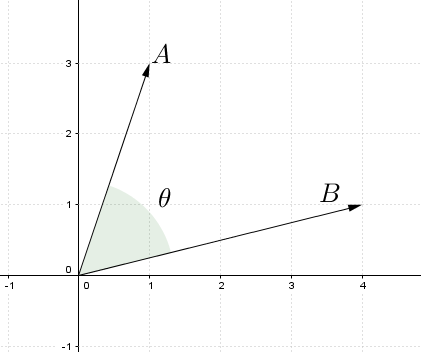
\includegraphics[width=0.4\linewidth]{img/vettori_angolo_theta.png}
\end{center}

inizio a trovare l'angolo della prima coppia di vettori
\begin{enumerate}[label=\alph*.]
	\item $\cos (\theta) = \dfrac{1\cdot 1 + 0\cdot 1}{\sqrt{1^2+0^2}\cdot \sqrt{1^2+1^2}} = \frac{1}{\sqrt{2}}$
	\item $\cos (\theta) = \dfrac{1\cdot 1\sqrt{3}+ 0\cdot 1}{\sqrt{1^2+0^2}\cdot \sqrt{(\sqrt{3})^2+1^2}} = \frac{\sqrt{3}}{2}$
	\item $\cos (\theta) = \dfrac{1\cdot 1 + 0\cdot \sqrt{3}}{\sqrt{1^2+0^2}\cdot \sqrt{1^2+(\sqrt{3})^2}} = \frac{1}{2}$
	\item $\cos (\theta) = \dfrac{1\cdot (-1) + 0\cdot \sqrt{3}}{\sqrt{1^2+0^2}\cdot \sqrt{(-1)^2+(\sqrt{3})^2}} = -\frac{1}{2}$
	\item $\cos (\theta) = \dfrac{0\cdot \sqrt{3} + 1\cdot (-1)}{\sqrt{0^2+1^2}\cdot \sqrt{(\sqrt{3})^2+(-1)^2}} = -\frac{1}{2}$
\end{enumerate}
\pagebreak
\subsubsection{Esercizio 2} 
Trovare l'equazione parametrica passante per $P(2,3)$ e $Q(-1,2)$
\begin{center}
	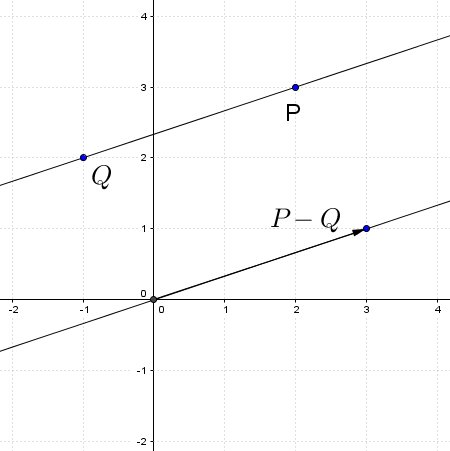
\includegraphics[width=0.4\linewidth]{img/vettori_rette_parametriche.png}
\end{center}
\begin{gather*}
	P-Q = (2-(-1), 3-2) = (3,1)\\
	...?
\end{gather*}

\pagebreak
\subsubsection{Esercizio 3} 
Trovare l'equazione della retta passante per $P(1,1,-1)$ e $Q(-2,1,3)$
\begin{gather*}
	P-Q = (3,0,-4) \qquad \text{trovo $P-Q$}\\
	(3,0,-4)t + (-2,1,3) \qquad \text{sommo $(P-Q)t$ ad un punto appartenente alla retta ($Q$ in questo caso)}\\\\
	x = 3t - 2 \\
	y = 1\\
	z = -4t + 3
\end{gather*}\\\\
\subsubsection{Esercizio 4}
Trovare l'equazione della retta perpendicolare a $P(1,-1)$ e passante per $Q(-5,3)$\\\\
Sapendo che un vettore $(x,y)$ è perpendicolare ad $(1,-1)$ sse $(1,-1)(x,y)=0 \to x-y+c=0$
\begin{gather*}
	x-y+c = 0 \\
	-5 - 3 + c = 0 \qquad \text{sostituisco con le coordinate del punto per il quale la retta passa}\\
	c=8 \qquad \text{e trovo $c$}\\\\
	x-y=-8 \qquad \text{equazione della retta perpendicolare}
\end{gather*}
Disegno esplicativo:
\begin{center}
	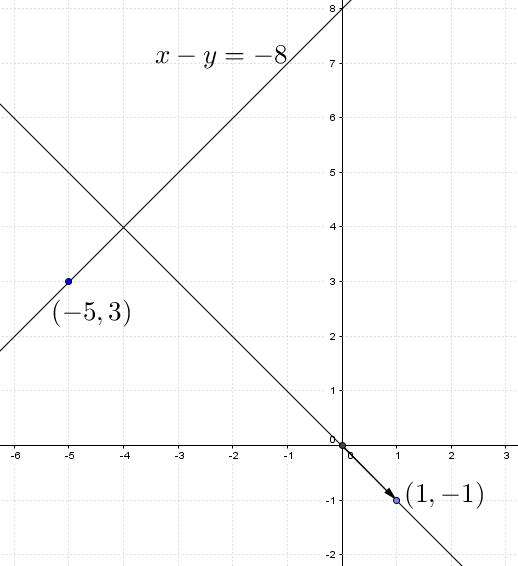
\includegraphics[width=0.5\linewidth]{img/vettori_rette_perpendicolari.png}
\end{center}
\pagebreak
\subsubsection{Esercizio 5}
Scrivere in forma cartesiana
\[
	(1,0)t + (0,3) = (x,y)
\]
\begin{gather*}
	x = 1\cdot t + 0 = t\\
	y = 0\cdot t + 3 = 3
\end{gather*}
\subsubsection{Esercizio 6}
Scrivere in forma parametrica
\[
	3x-2y+5=0
\]
Devo prendere un punto (\textit{vettore}) della retta parallela passante per l'origine
\begin{gather*}
	t(2,3) + \left( 0, \dfrac{5}{2} \right) = (x,y)
\end{gather*}
Disegno esplicativo:
\begin{center}
	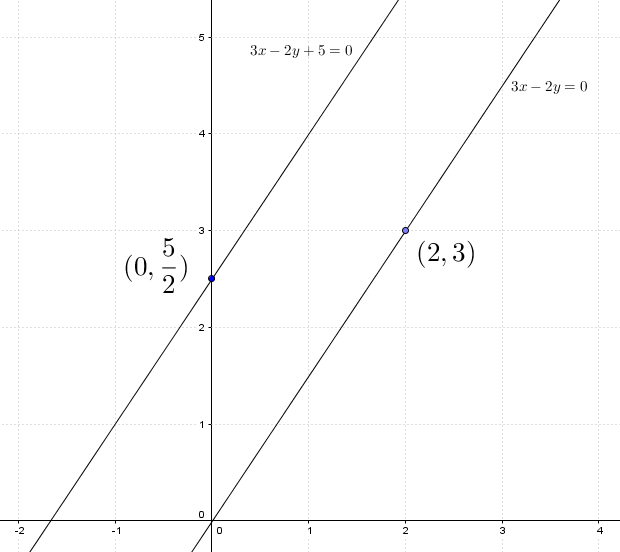
\includegraphics[width=0.5\linewidth]{img/vettori_forma_parametrica.png}
\end{center}


\newpage
\subsection{Spazi vettoriali}
\subsubsection{Esercizio 1}
Quali dei seguenti insiemi sono sottospazi vettoriali:
\begin{gather*}
	v_1 = \{ (x,y,x) \in \ins{R}^3 \qquad x=y=z \} \\
	v_2 = \{ (x,y,x) \in \ins{R}^3 \qquad x=4 \} \\
	v_3 = \{ (x,y,x) \in \ins{R}^3 \qquad z=x^2 \} \\
	v_4 = \{ (x,y,x) \in \ins{R}^3 \qquad (x-y)^2=0 \}
\end{gather*}

\noindent\textbf{Svolgimento} $v_1$: è sottospazio
\begin{itemize}
	\item verifico che $0 \in v_1$:
	\[
		\{ 0 \in v_1 \} \checkmark
	\]
	\item verifico che il prodotto per uno scalare stia ancora in $v_1$:
	\begin{gather*}
		(a,b,c) \in v_1 \qquad \lambda \in v_1\\\\
		\lambda(a,b,c) \in v_1 ?\\
		a=b=c \\
		\lambda(a,b,c) = (\lambda a , \lambda b , \lambda c) = \lambda a = \lambda b = \lambda c \checkmark
	\end{gather*}
	\item verifico che la somma resti in $v_1$:
	\begin{gather*}
		(a,b,c),(m,n,p) \in v_1\\\\
		(a+m,b+n,c+p) \in v_1 ?\\
		\begin{rcases*}
			a = b = c \\
			m = n = p
		\end{rcases*}
		a + m = b + n = c + p \in v_1 \checkmark  
	\end{gather*}
\end{itemize}

\noindent\textbf{Svolgimento} $v_2$: non è sottospazio
\begin{itemize}
	\item verifico che $0 \in v_2$:
	\[
		\{ 0 \notin v_1 \} \crossmark
	\]
\end{itemize}

\noindent\textbf{Svolgimento} $v_3$: non è sottospazio
\begin{itemize}
	\item verifico che $0 \in v_3$:
	\[
		\{ 0 \in v_1 \} \checkmark
	\]
	\item verifico che la somma resti in $v_3$:
	\begin{gather*}
	(a,b,c) \in v_3 \Leftrightarrow a=c^2\\
	(a,b,a^2) \in v_3\\\\
	\begin{rcases*}
		x=(2,3,4) \in v_3 \\
		y = (3,2,9) \in v_3
	\end{rcases*}
	x+y=(5,5,13) \notin v_3 \crossmark
	\end{gather*}
\end{itemize}

\noindent\textbf{Svolgimento} $v_4$: per casa


\newpage
\subsubsection{Esercizio 2}
Trovare una base dello spazio vettoriale $(\ins{C}, +)$ sul campo numerico $(\ins{C}, +, \cdot)$
\begin{gather*}
	\text{1 e $i$ sono linearmente indipendenti?}\\\\
	\underbracket{(-i)}_{\mathclap{\text{scalre su \ins{C}}}}\cdot 1 + \overbracket{1}^{\mathclap{\text{scalare su \ins{C}}}}\cdot i = 0 \qquad \text{non sono linearmente indipendenti}
\end{gather*}
Una delle basi è
\begin{gather*}
	1: \text{perché } 1 \cdot(a+bi) = a + bi \text{ che è un numero in \ins{C}} \\
	oppure \\
	i: \text{perché } i \cdot(a+bi) = ai - b \text{ che è un numero in \ins{C}}
\end{gather*}

\subsubsection{Esercizio 3}
Trovare una base dello spazio vettoriale $(\ins{C}, +)$ sul campo numerico $(\ins{R}, +, \cdot)$\\\\
Una delle basi è $(1,i)$ perché sono linearmente indipendenti, in quanto in \ins{R} non esistono due scalari diversi da zero che annullino $a + bi$.


\subsubsection{Esercizio 4}
Estendere ad una base di $\ins{R}^3$:
\begin{gather*}
	v_1 = (1,1,1) \qquad v_2 = (0,1,2) \qquad v_3 = (0,1,0)	\\\\
	\lambda(1,1,1) + \mu(0,1,2) + \delta(0,1,0) =\\
	\lambda + \delta = 0 \Rightarrow \delta = -\lambda\\
	\lambda + \mu = 0 \Rightarrow \mu = -\lambda \\
	\lambda + \mu = 0 \Rightarrow \lambda = - \mu
\end{gather*}
sono linearmente indipendenti in quanto non esistono scalari diversi da 0 che li annullino.

\subsubsection{Esercizio 5}
Siano
\begin{gather*}
	V_1 = \{ t(1,1,1) : t \in \ins{R} \} \\
	V_2 = \{ s(1,0,1) : s \in \ins{R} \}
\end{gather*}
e $V_1,V_2 \subseteq \ins{R}^3$.\\[2mm]
$V_1 \cup V_2$ è sottospazio vettoriale di $\ins{R}^3$?\\

\noindent\textbf{Svolgimento} $V_1 \cup V_2$: non è sottospazio
\begin{itemize}
	\item verifico che $0 \in v_3$:
	\[
		\{ 0 \in V_1 \cup V_2 \} \checkmark
	\]
	\item verifico che la somma resti in $V_1 \cup V_2$:
	\begin{gather*}
		a,b \in V_1 \cup V_2 \Leftrightarrow a + b \in V_1 \cup V_2 \; ? \\
		(1,1,1)+(1,0,1) \in V_1 \cup V_2 \; ? \\
		(2,1,2) \notin V_1 \cup V_2 \crossmark
	\end{gather*}
\end{itemize}
La somma non sta in $V_1 \cup V_2$ perché non soddisfa le condizioni iniziali.\\
Il punto $(1,1,1)$ equivale a scrivere $x=y=z$, e possiamo subito notare che su $(2,1,2)$ le variabili $x,y,z$ non sono uguali.


\subsubsection{Esercizio 6}
Sia $P^5[x]$ lo spazio dei polinomi reali di grado $\leq 5$. Qual è lo spazio generato dai vettori:
\begin{itemize}
	\item $-x^3 + 4x^2$ 
	\item $5x^3$
	\item $-3x^2$
\end{itemize}
Svolgimento:
\[
	\{ \lambda(-x^3 + 4x^2) + \mu(5x^3) + \delta(-3x^2) \quad \text{con } \lambda, \mu, \delta \in \ins{R}\}
\]
Se $\lambda = \mu = \delta = 1$ allora
\[
	-x^3 + 4x^2 + 5x^3 - 3x^2 = 4x^3 + x^2
\]
ma $4x^3$ può essere visto come una combinazione lineare di
\[
	\varepsilon x^3 \quad \text{con } \varepsilon = 4
\]
Quindi i vettori utili alle generazione di tutto lo spazio sono $5x^3$ e $-3x^2$, che a loro volta possono generare anche il vettore $-x^3 + 4x^2$. \\[2mm]
Questi due vettori tuttavia possono essere visti a loro volta come combinazioni lineari di altri vettori, e quindi possiamo verificare che una base di $P^5[x]$ può essere 
\[
	\{  \mu(5x^3) + \delta(-3x^2) \quad \text{con } \mu, \delta \in \ins{R} \} \\
\]
ma essendo combinazione lineare di 
\[
	x^2 ,\; x^3
\] possiamo assumere come base proprio $x^2, x^3$.

\subsubsection{Esercizio 7}
Sia $M(2\times 2), \ins{R}$ lo spazio delle matrici $2\times 2$.\\[2mm]
Dimostrare che le seguenti matrici siano una base di $M(2\times 2), \ins{R}$:
\[
	\begin{bmatrix}
		1 & 0 \\ 0 & 1
	\end{bmatrix}
	,
	\begin{bmatrix}
		1 & 2 \\ 0 & 0
	\end{bmatrix}
	,
	\begin{bmatrix}
		1 & 2 \\ 3 & 0
	\end{bmatrix}
	,
	\begin{bmatrix}
		1 & 2 \\ 3 & 4
	\end{bmatrix}
\]
Svolgimento:
\begin{gather*}
	\begin{bmatrix}
		a & b \\ c & d
	\end{bmatrix}
	=
	a
	\begin{bmatrix}
		1 & 0 \\ 0 & 0
	\end{bmatrix}
	+
	b
	\begin{bmatrix}
		0 & 1 \\ 0 & 0
	\end{bmatrix}
	+
	c
	\begin{bmatrix}
		0 & 0 \\ 1 & 0
	\end{bmatrix}
	+
	d
	\begin{bmatrix}
		0 & 0 \\ 0 & 1
	\end{bmatrix}	
\end{gather*}
Controllo che siano linearmente indipendenti:
\begin{gather*}
	c_1
	\begin{bmatrix}
		1 & 0 \\ 0 & 1
	\end{bmatrix}
	+
	c_2
	\begin{bmatrix}
		1 & 2 \\ 0 & 0
	\end{bmatrix}
	+
	c_3
	\begin{bmatrix}
		1 & 2 \\ 3 & 0
	\end{bmatrix}
	+
	c_4
	\begin{bmatrix}
		1 & 2 \\ 3 & 4
	\end{bmatrix} \\\\
	\begin{cases*}
		c_1 + c_2 + c_3 + c_4 = 0 \\
		2c_2 + 2c_3 + 2c_4 = 0 \\
		3c_3 + 3c_4 = 0 \\
		c_1 + 4c_4 = 0
	\end{cases*}
	\to c_1 = c_2 = c_3 = c_4 = 0
\end{gather*}
Non esistono valori diversi da 0 di $c_1,c_2,c_3,c_4$ per cui il sistema sia verificato. Le matrici sono dunque linearmente indipendenti e sono una base di $M(2\times 2), \ins{R}$.

\tright{20-11-2015}
\subsubsection{Esercizio 8}
Dato un insieme $X$ e un campo \ins{K}:
\[
	A = \{ f: X \longmapsto \ins{K} \}
\]
Dimostrare che è uno spazio vettoriale rispetto alle operazioni
\begin{itemize}
	\item assioma 1: $(f+g) + h = f + (g+h)$
		\begin{gather*}
			\begin{split}
				(f+g)x + h(x) &= (f+(g+h))(x) \\
				f(x) + g(x) + h(x) &= f(x) + (g+h)(x) \\
				&= f(x) + g(x) + h(x) \checkmark
			\end{split}
		\end{gather*}
		\item assioma 2: $f + g = g + f $
			\begin{gather*}
			\begin{split}
				f(x) + g(x) &= g(x) + f(x) \\
				&= f(x) + g(x) \checkmark
			\end{split}
			\end{gather*}
		\item assioma 3: elemento neutro: $ \bigcirc: X \longmapsto \ins{K} $
			\begin{gather*}
				\begin{split}
					(f + \bigcirc) &= f(x) + \bigcirc(x) \\
					&= f(x) \checkmark
				\end{split}
			\end{gather*}
		\item assioma 4: $ -f: X \longmapsto \ins{K} $
			\begin{gather*}
				\begin{split}
					(-f(x)) = -f(x) \checkmark
				\end{split}
			\end{gather*}
		\item assioma 5: $ (\lambda\mu)f = \lambda(\mu f) \qquad \lambda,\mu \in \ins{K}$
			\begin{gather*}
				\begin{split}
					(\lambda\mu)f(x) &= \lambda(\mu f(x)) \\
					&= \lambda \left[ (\mu f)(x) \right] \checkmark
				\end{split}
			\end{gather*}
		\item assioma 6: $ \lambda(f+g) = \lambda f + \lambda g \qquad \lambda \in \ins{K}$
			\begin{gather*}
				\begin{split}
					\lambda(f+g)(x) &= \lambda f(x) + \lambda g(x) \\
					&= \lambda \left[ f(x) + g(x) \right] \\
					&= (\lambda f + \lambda g)(x) \checkmark
				\end{split}
			\end{gather*}
		\item assioma 7: $ (\lambda + \mu)f = \lambda f + \mu f\qquad \lambda,\mu \in \ins{K}$
			\begin{gather*}
				\begin{split}
					(\lambda + \mu)f(x) &= \lambda f(x) + \mu f(x) \\
					&= (\lambda f + \lambda g)(x) \checkmark
				\end{split}
			\end{gather*}
\end{itemize}

\newpage
\subsubsection{Esercizio 9}
Verificare che le seguenti funzioni siano lineari:
\begin{enumerate}[label=\alph*)]
	\item $f: \ins{R} \longmapsto \ins{R} \qquad x \to \sin(x)$
	\item $f: \ins{R}^2 \longmapsto \ins{R} \qquad (x,y) \to (2x+y)$
	\item $f: \ins{R}^2 \longmapsto \ins{R}^3 \qquad (x,y) \to (-x,-x+y,-x+y^2)$
\end{enumerate}
Una funzione è lineare quando:
\begin{gather*}
	f(x+y)= f(x) + f(y) \\
	f(\lambda x) = \lambda f(x)
\end{gather*}
\textbf{Svolgimento}\\
a) - non lineare
\begin{gather*}
	\begin{split}
		\sin(\frac{\pi}{2} + \frac{\pi}{2}) &= \sin(\frac{\pi}{2}) + \sin(\frac{\pi}{2}) \\
		0 &= 1 + 1 \\
		0 &= 2 \crossmark
	\end{split}
\end{gather*}
b) - lineare
\begin{gather*}
	\forall (x,y),(a,b) \in \ins{R}^2\\\\
	\begin{split}
		f\left((x,y) + (a,b) \right) &= f(x,y) + f(a,b) \\
		&= f(x+a, y+b) \\\\
		2x + y + 2a + b &= 2(x+a) + y + b \checkmark
	\end{split}
\end{gather*}
b) - non lineare
\begin{gather*}
	\begin{split}
		f\bigr((0,1) + (0,2)\bigr) &= f(0,3) = (0,3,9) \\
		f(0,1) + f(0,2) &= (0,1,1) + (0,2,4) = (0,3,5) \crossmark
	\end{split}
\end{gather*}

\newpage
\subsubsection{Esercizio 10 - App. lineari}
Data un'applicazione lineare
\[
	f: \ins{R}^3 \longmapsto \ins{R}^3
\]
che definisce una matrice $3 \times 3$, determinare la dimensione del $\ker{f}$.\\[2mm]
Le basi sono quelle canoniche di $\ins{R}^3$.\\[2mm]
Le immagini delle basi sono
\begin{gather*}
	f(e_1) = (1,0,2) \\
	f(e_2) = (-1,1,0) \\
	f(e_3) = (0,1,-1)
\end{gather*}
e determinano la matrice
\[
	\begin{bmatrix}
		1 & -1 & 0 \\
		0 & 1 & 1 \\
		2 & 0 & -1
	\end{bmatrix}
	\begin{bmatrix}
		c_1 \\ c_2 \\ c_3
	\end{bmatrix}
	=
	\begin{bmatrix}
		c_1 - c_2 \\ c_2 + c_3 \\ 2c_1 - c_3
	\end{bmatrix}
\]
trovo
\[
	\begin{split}
		f(c_1e_1 + c_2e_2 + c_3e_3) &= c_1(w_1 + 2w_3) + c_2(-w_1 + w_2) + c_3(w_2 - w_3) \\
		&= w_1(c_1 - c_2) + w_2(c_2 + c_3) + w_3(2c_1 - c_3)
	\end{split}
\]
\begin{gather*}
	\ker{f} = \{ v \in \ins{R}^3 : f(v) = 0 \} \qquad M\begin{bmatrix}x \\ y \\z\end{bmatrix} = 0 \to \begin{bmatrix}x \\ y \\z\end{bmatrix} = \begin{bmatrix}0\\0\\0\end{bmatrix} \\\\
	\dim{V} = \dim{\ker{f}} + \dim{\imm{f}} \\
	\dim{\ker{f}} = 0 \\
	\dim{\imm{f}} = 3
\end{gather*}
Possiamo quindi concludere che questa applicazione lineare è isomorfa.
\end{document}
